\part{Lecture 07: Planning and Learning with Tabular Methods}
\title[RL Lecture 07]{Lecture 07: Planning and Learning \\with Tabular Methods}  
\date{}  
\frame{\titlepage} 

%%%%%%%%%%%%%%%%%%%%%%%%%%%%%%%%%%%%%%%%%%%%%%%%%%%%%%%%%%%%%
%% Recall: RL Agent Taxonomy%%
%%%%%%%%%%%%%%%%%%%%%%%%%%%%%%%%%%%%%%%%%%%%%%%%%%%%%%%%%%%%%
\frame{\frametitle{Recap: RL Agent Taxonomy}
\begin{figure}
	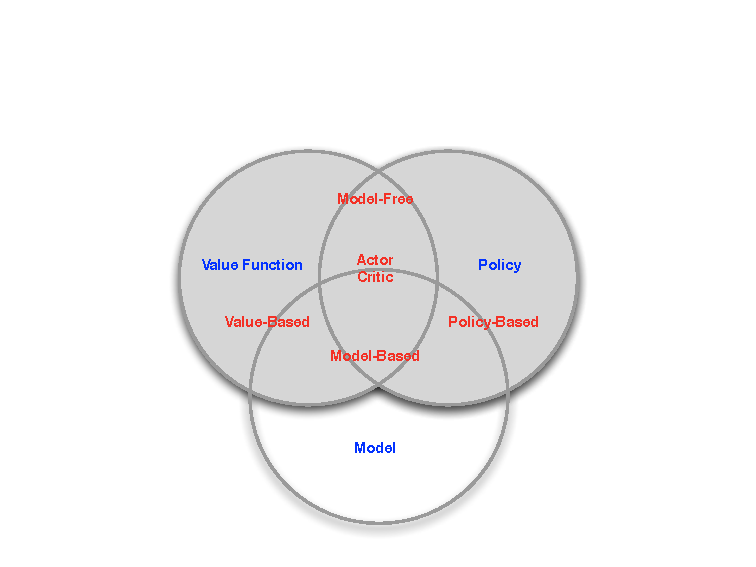
\includegraphics[width=5.5cm]{fig/lec01/RL_Agent_Taxonomy.pdf}
	\caption{Main categories of reinforcement learning algorithms\\  \SilverLectureSource}
\end{figure}
\begin{itemize}
	\item Up to now: independent usage of model-free and model-based RL
	\item Today: integrating both strategies (on finite  state \& action spaces)
\end{itemize}
}

%%%%%%%%%%%%%%%%%%%%%%%%%%%%%%%%%%%%%%%%%%%%%%%%%%%%%%%%%%%%%%%%%%
\section{Repetition: Model-based and Model-free RL} 
%%%%%%%%%%%%%%%%%%%%%%%%%%%%%%%%%%%%%%%%%%%%%%%%%%%%%%%%%%%%%%%%%%
\begin{frame}
\frametitle{Table of Contents}
\tableofcontents
\end{frame}

%%%%%%%%%%%%%%%%%%%%%%%%%%%%%%%%%%%%%%%%%%%%%%%%%%%%%%%%%%%%%
%% Model-based RL %%
%%%%%%%%%%%%%%%%%%%%%%%%%%%%%%%%%%%%%%%%%%%%%%%%%%%%%%%%%%%%%
\frame{\frametitle{Model-based RL}
\begin{itemize}
	\item \hl{Plan/predict} value functions and/or policy from a model.
	\item Requires an a priori model or to learn a model from experience.
	\item Solves control problems by planning algorithms such as
	\begin{itemize}
		\item Policy iteration or
		\item Value iteration.
	\end{itemize}
\end{itemize}
\begin{figure}
	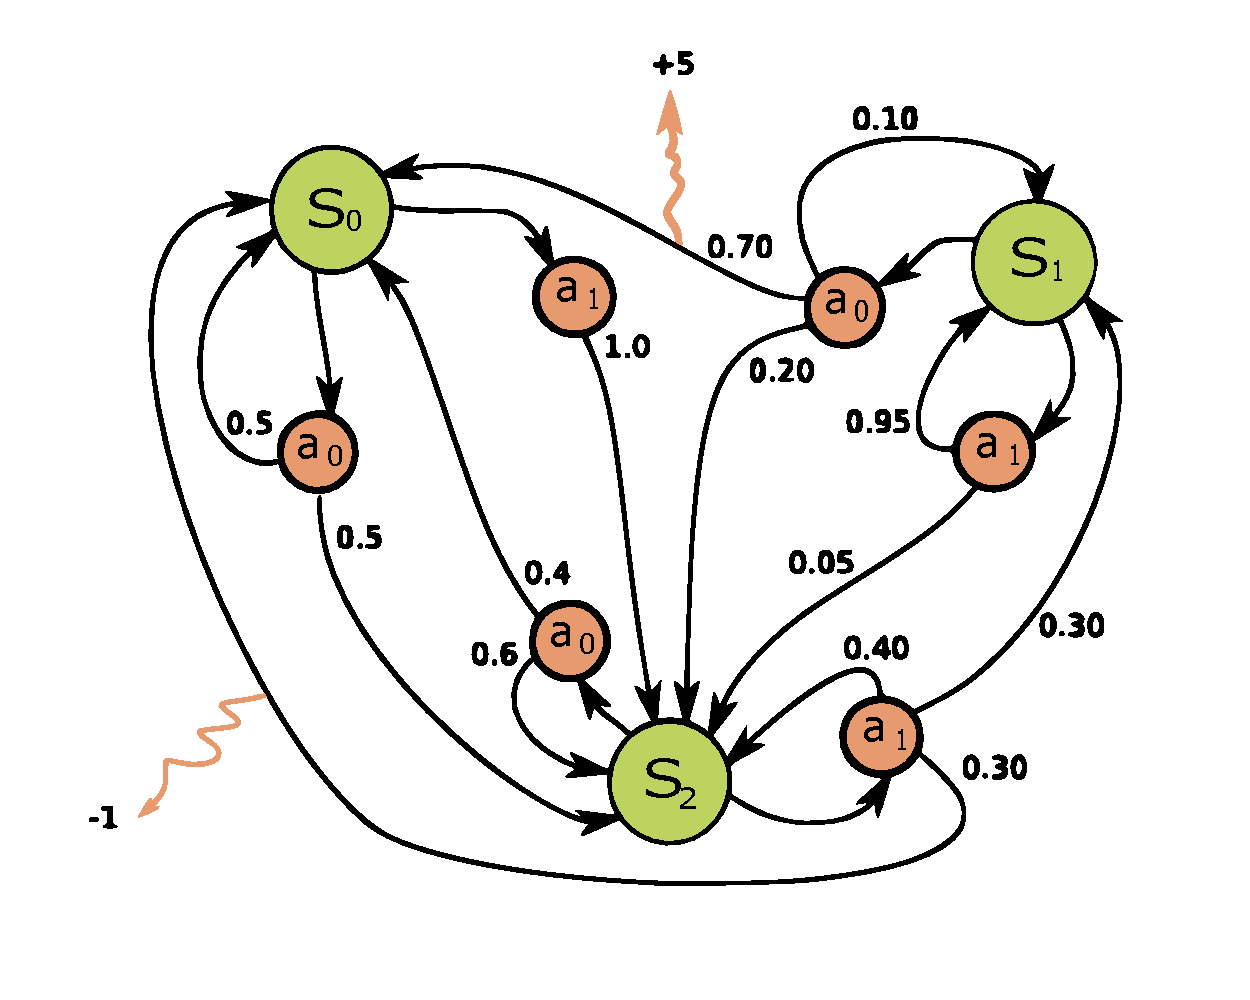
\includegraphics[width=5.5cm]{fig/lec07/Markov_Decision_Process.pdf}
	\caption{A model for discrete state and action space problems is generally an MDP (source: \href{https://commons.wikimedia.org/wiki/File:Markov_Decision_Process.svg}{www.wikipedia.org},  by \href{https://commons.wikimedia.org/wiki/User:Waldoalvarez}{Waldoalvarez} \href{https://creativecommons.org/licenses/by-sa/4.0/deed.en}{CC BY-SA 4.0})}
	\label{fig:Markov_Decision_Process}
\end{figure}
}

%%%%%%%%%%%%%%%%%%%%%%%%%%%%%%%%%%%%%%%%%%%%%%%%%%%%%%%%%%%%%
%% What is a Model? %%
%%%%%%%%%%%%%%%%%%%%%%%%%%%%%%%%%%%%%%%%%%%%%%%%%%%%%%%%%%%%%
\frame{\frametitle{What is a Model?}
\begin{itemize}
	\item A model $\mathcal{M}$ is an MDP tuple $\left\langle\mathcal{X}, \mathcal{U}, \bm{\mathcal{P}}, \mathcal{R}, \gamma \right\rangle$. \pause
	\item In particular, we require the  
	\begin{itemize}
		\item state-transition probability
	\begin{equation}
		\bm{\mathcal{P}} = \Pb{\bm{X}_{k+1}=\bm{x}_{k+1}|\bm{X}_k=\bm{x}_k, \bm{U}_k=\bm{u}_k}
	\end{equation}
	\item and the reward probability
	\begin{equation}
		\mathcal{R} = \Pb{R_{k+1}=r_{k+1}|\bm{X}_k=\bm{x}_k, \bm{U}_k=\bm{u}_k}\,.
	\end{equation}
	\end{itemize}\pause
	\item State space $\mathcal{X}$ and action space $\mathcal{U}$ is assumed to be known.\pause
	\item Discount factor $\gamma$ might be given by environment or engineer's choice. \pause
	\item What kind of model is available?
	\begin{itemize}
	\item If $\mathcal{M}$ is perfectly known a priori: \hl{true MDP}.
	\item If $\hat{\mathcal{M}}\approx \mathcal{M}$ needs to be learned: \hl{approximated MDP}.
\end{itemize}
\end{itemize}

}

%%%%%%%%%%%%%%%%%%%%%%%%%%%%%%%%%%%%%%%%%%%%%%%%%%%%%%%%%%%%%
%% Model Learning / Identification %%
%%%%%%%%%%%%%%%%%%%%%%%%%%%%%%%%%%%%%%%%%%%%%%%%%%%%%%%%%%%%%
\frame{\frametitle{Model Learning / Identification}
\begin{itemize}
	\item Ideally, the model $\mathcal{M}$ is exactly known a priori (e.g., gridworld case). \pause
	\item On the contrary, a model might be too complex to derive or not exactly available (e.g., real physical systems). \pause
	\begin{itemize}
		\item \hl{Objective: estimate model $\hat{\mathcal{M}}$ from experience $\left\{X_0, U_0,R_1,\ldots,X_T\right\}$.} \pause
	\end{itemize}
	\item This is a supervised learning / system identification task:
	\begin{align*}
		\left\{X_0, U_0\right\}&\rightarrow\left\{X_1, R_1\right\}\\
		&\vdots\\
		\left\{X_{T-1}, U_{T-1}\right\}&\rightarrow\left\{X_{T}, R_{T}\right\}
	\end{align*}\pause\vspace{-0.2cm} 
	\item Simple tabular / look-up table approach (with $n(x,u)$ visit count):
	\begin{equation}
		\begin{split}
		\hat{p}_{xx'}^u&=\frac{1}{n(x,u)}\sum_{k=0}^{T} 1(X_{k+1}=x'|X_{k}=x, U_k=u),\\
		\hat{\mathcal{R}}_{x}^u&=\frac{1}{n(x,u)}\sum_{k=0}^{T} 1(X_{k}=x|U_k=u) r_{k+1}.
	\end{split}
	\label{eq:dist_model}
	\end{equation}
\end{itemize}
}

%%%%%%%%%%%%%%%%%%%%%%%%%%%%%%%%%%%%%%%%%%%%%%%%%%%%%%%%%%%%%
%% Distribution vs. Sample Models %%
%%%%%%%%%%%%%%%%%%%%%%%%%%%%%%%%%%%%%%%%%%%%%%%%%%%%%%%%%%%%%
\frame{\frametitle{Distribution vs. Sample Models}
\begin{itemize}
	\onslide<1->{\item A model based on $\bm{\mathcal{P}}$ and $\mathcal{R}$ is called a \hl{distribution model}.
	\begin{itemize}
		\item Contains descriptions of all possibilities by random distributions. 
		\item Has full explanatory power, but is still rather complex to obtain. 
	\end{itemize}}
	\onslide<2->{\item Alternatively, use \hl{sample models} to receive realization series.
	\begin{itemize}
		\item Remember black jack examples: easy to sample by simulation but hard to model a full distributional MDP. 
	\end{itemize}}
\end{itemize}
\onslide<1->{\begin{figure}
	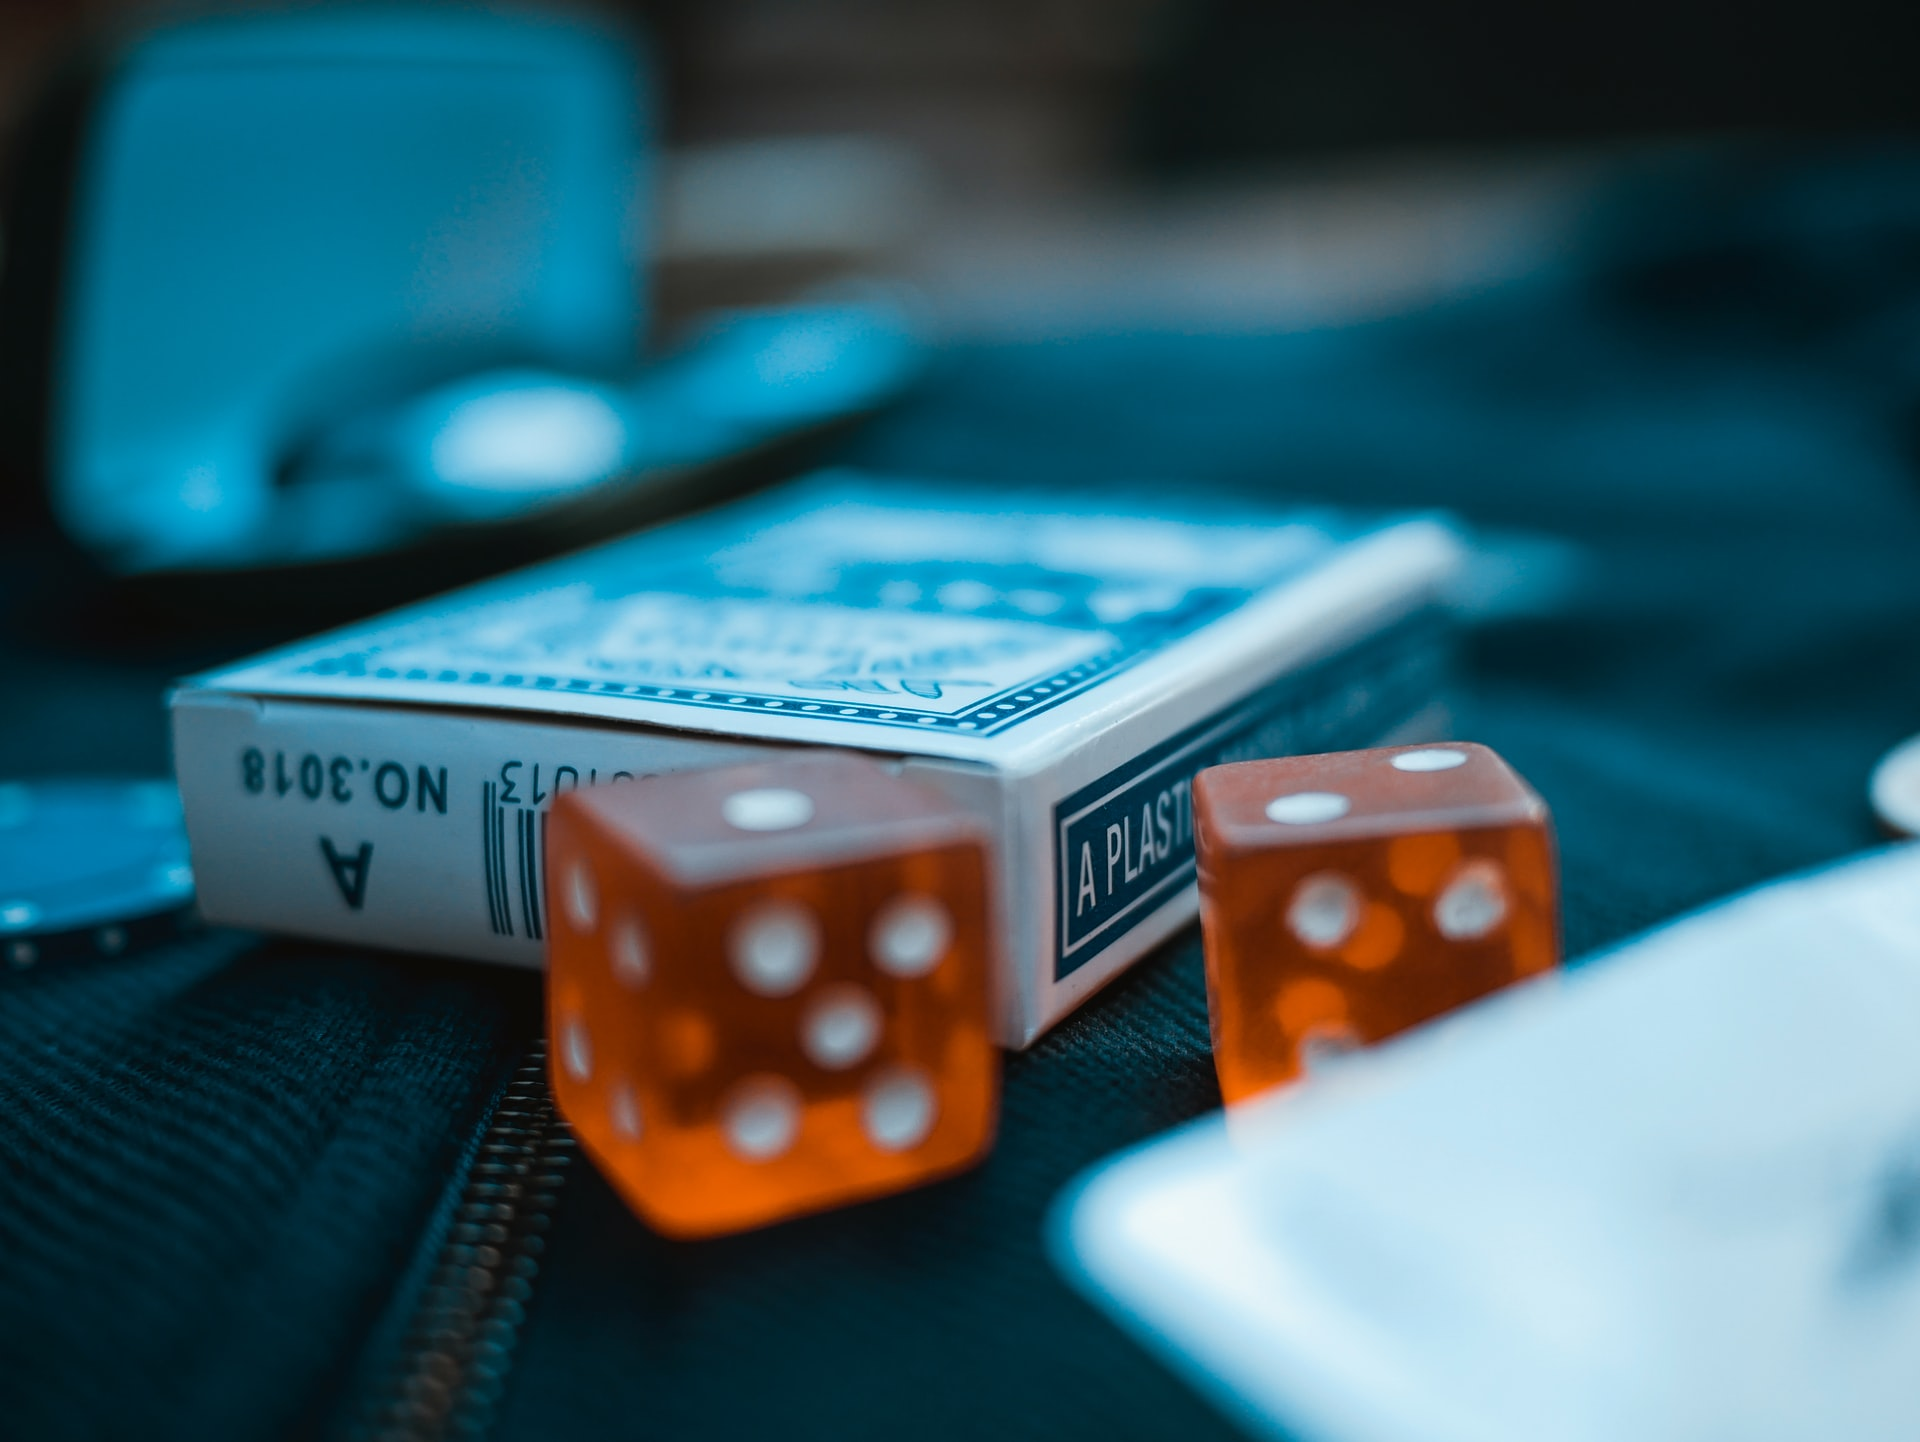
\includegraphics[width=5.0cm]{fig/lec07/cards_dice.jpg}
	\caption{Depending on the application distribution models are easily available or not (source: Josh Appel on \href{https://unsplash.com/photos/PHwdpTVUlXw}{Unsplash})}
\end{figure}}
}

%%%%%%%%%%%%%%%%%%%%%%%%%%%%%%%%%%%%%%%%%%%%%%%%%%%%%%%%%%%%%
%% Model-free RL %%
%%%%%%%%%%%%%%%%%%%%%%%%%%%%%%%%%%%%%%%%%%%%%%%%%%%%%%%%%%%%%
\frame{\frametitle{Model-free RL}
\begin{itemize}
	\item \hl{Learn} value functions and/or policy directly from experience.
	\item Requires no model at all (policy can be considered an implicit model). \pause
	\item Solves control problems by learning algorithms such as
	\begin{itemize}
		\item Monte-Carlo,
		\item Sarsa or
		\item $Q$-learning.
	\end{itemize}
\end{itemize}\pause
\begin{figure}
	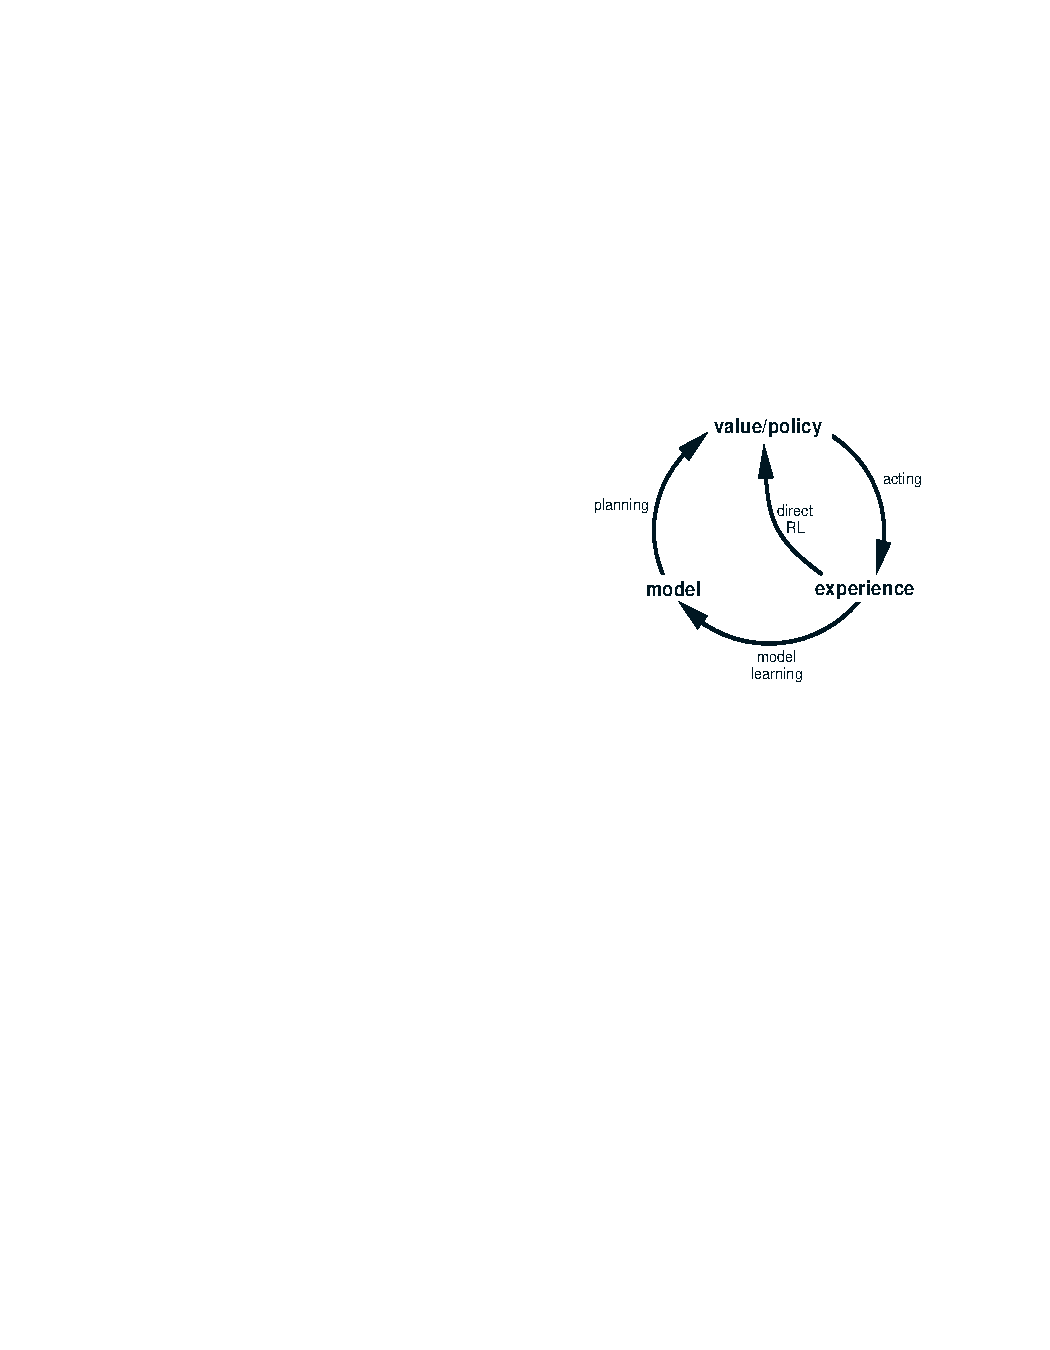
\includegraphics[width=4.5cm]{fig/lec07/direct_indirect_RL.pdf}
	\caption{If a perfect a priori model is not available, RL can be realized directly or indirectly (source: R. Sutton and G. Barto, Reinforcement learning: an introduction, 2018, \href{https://creativecommons.org/licenses/by-nc-nd/2.0/}{CC BY-NC-ND 2.0})}
	\label{fig:direct_indirect_RL}
\end{figure}
}

%%%%%%%%%%%%%%%%%%%%%%%%%%%%%%%%%%%%%%%%%%%%%%%%%%%%%%%%%%%%%
%% Advantages and Drawbacks: Model-free vs. Model-based RL %%
%%%%%%%%%%%%%%%%%%%%%%%%%%%%%%%%%%%%%%%%%%%%%%%%%%%%%%%%%%%%%
\frame{\frametitle{Advantages \& Drawbacks: Model-free vs. Model-based RL }
\onslide<1->{Pro model-based / indirect RL:
\begin{itemize}
	\item Efficiently uses limited amount of experience (e.g., by replay).  
	\item Allows integration of available a priori knowledge. 
	\item Learned models might be re-used for other tasks (e.g., monitoring).
\end{itemize}}
\vspace{0.25cm}
\onslide<2->{Pro model-free / direct RL:
\begin{itemize}
	\item Is simpler to implement (only one task, not two consequent ones).
	\item Not affected by model bias / error during model learning.
\end{itemize}}
\onslide<1->{\begin{figure}
	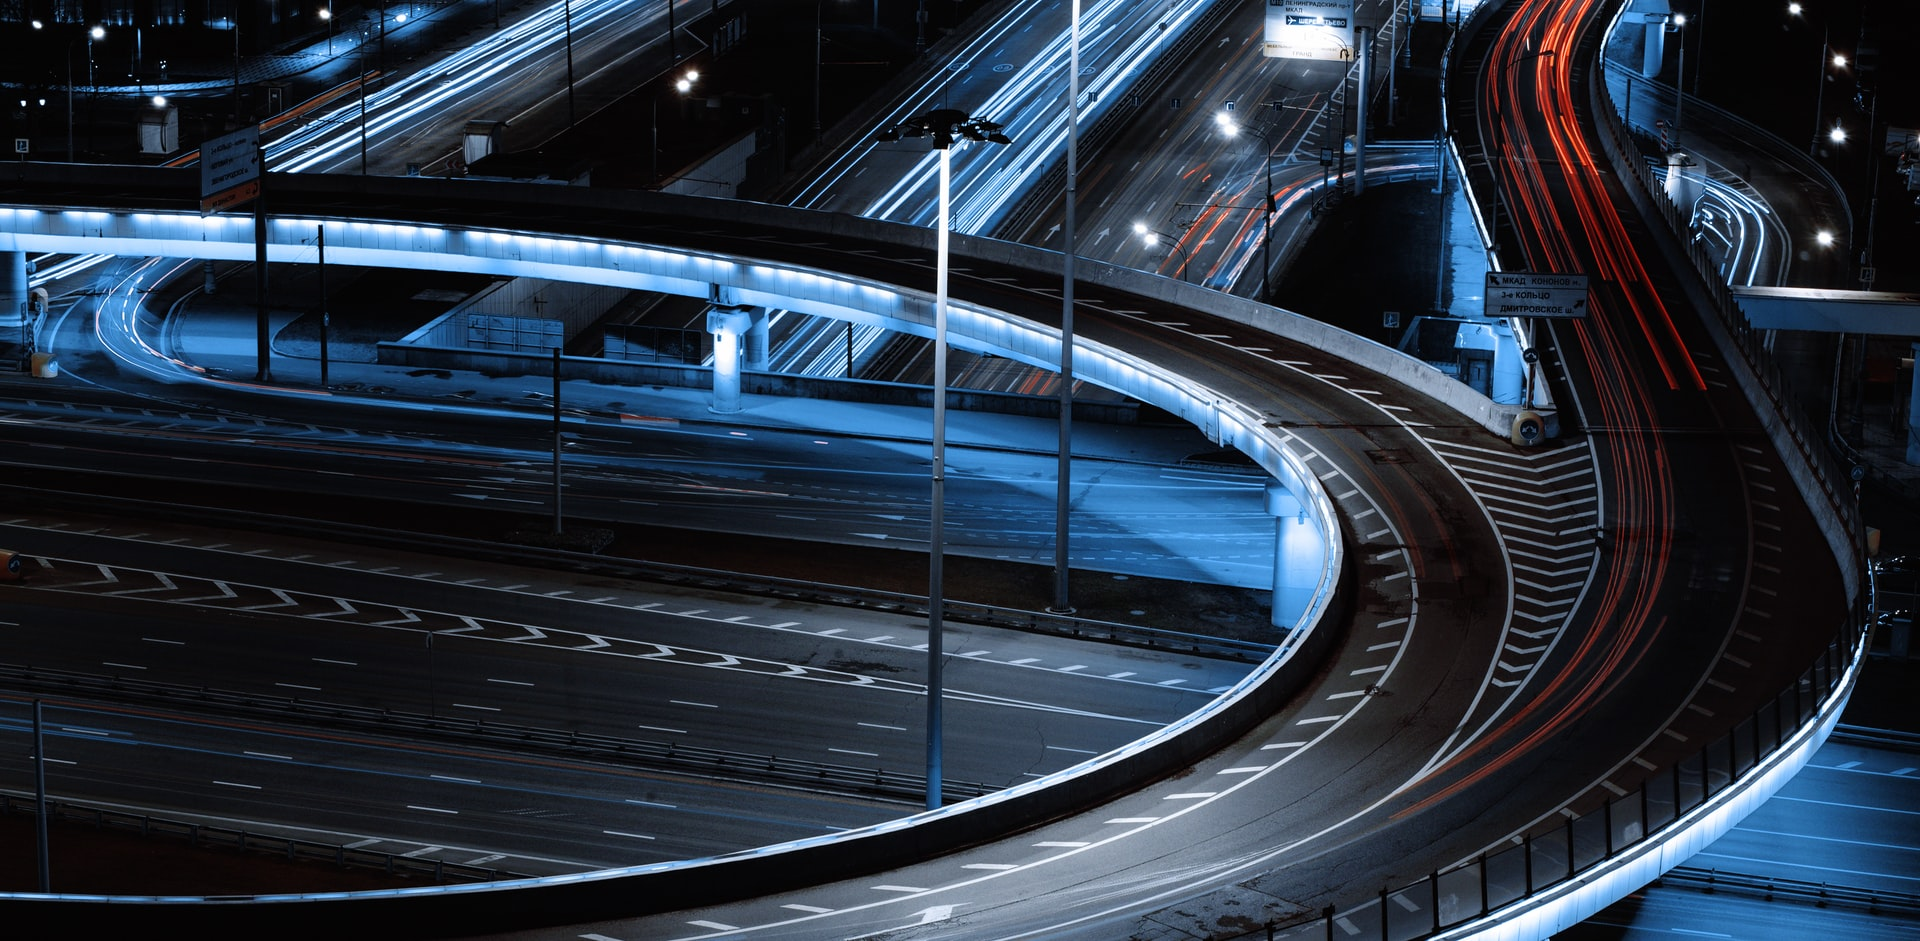
\includegraphics[width=7.0cm]{fig/lec07/crossroads.jpg}
	\caption{What way is better? (source: Mike Kononov on \href{https://unsplash.com/photos/FY0nQ-I3H_U}{Unsplash})}
\end{figure}}
}

%%%%%%%%%%%%%%%%%%%%%%%%%%%%%%%%%%%%%%%%%%%%%%%%%%%%%%%%%%%%%%%%%%
\section{Dyna: Integrated Planning, Acting and Learning} 
%%%%%%%%%%%%%%%%%%%%%%%%%%%%%%%%%%%%%%%%%%%%%%%%%%%%%%%%%%%%%%%%%%
\begin{frame}
\frametitle{Table of Contents}
\tableofcontents[currentsection]
\end{frame}

%%%%%%%%%%%%%%%%%%%%%%%%%%%%%%%%%%%%%%%%%%%%%%%%%%%%%%%%%%%%%
%% The General Dyna Architecture (1)%%
%%%%%%%%%%%%%%%%%%%%%%%%%%%%%%%%%%%%%%%%%%%%%%%%%%%%%%%%%%%%%
\frame{\frametitle{The General Dyna Architecture (1)}
\begin{itemize}
	\item Proposed by R. Sutton in 1990's
	\item General framework with many different implementation variants
\end{itemize}
\begin{figure}
	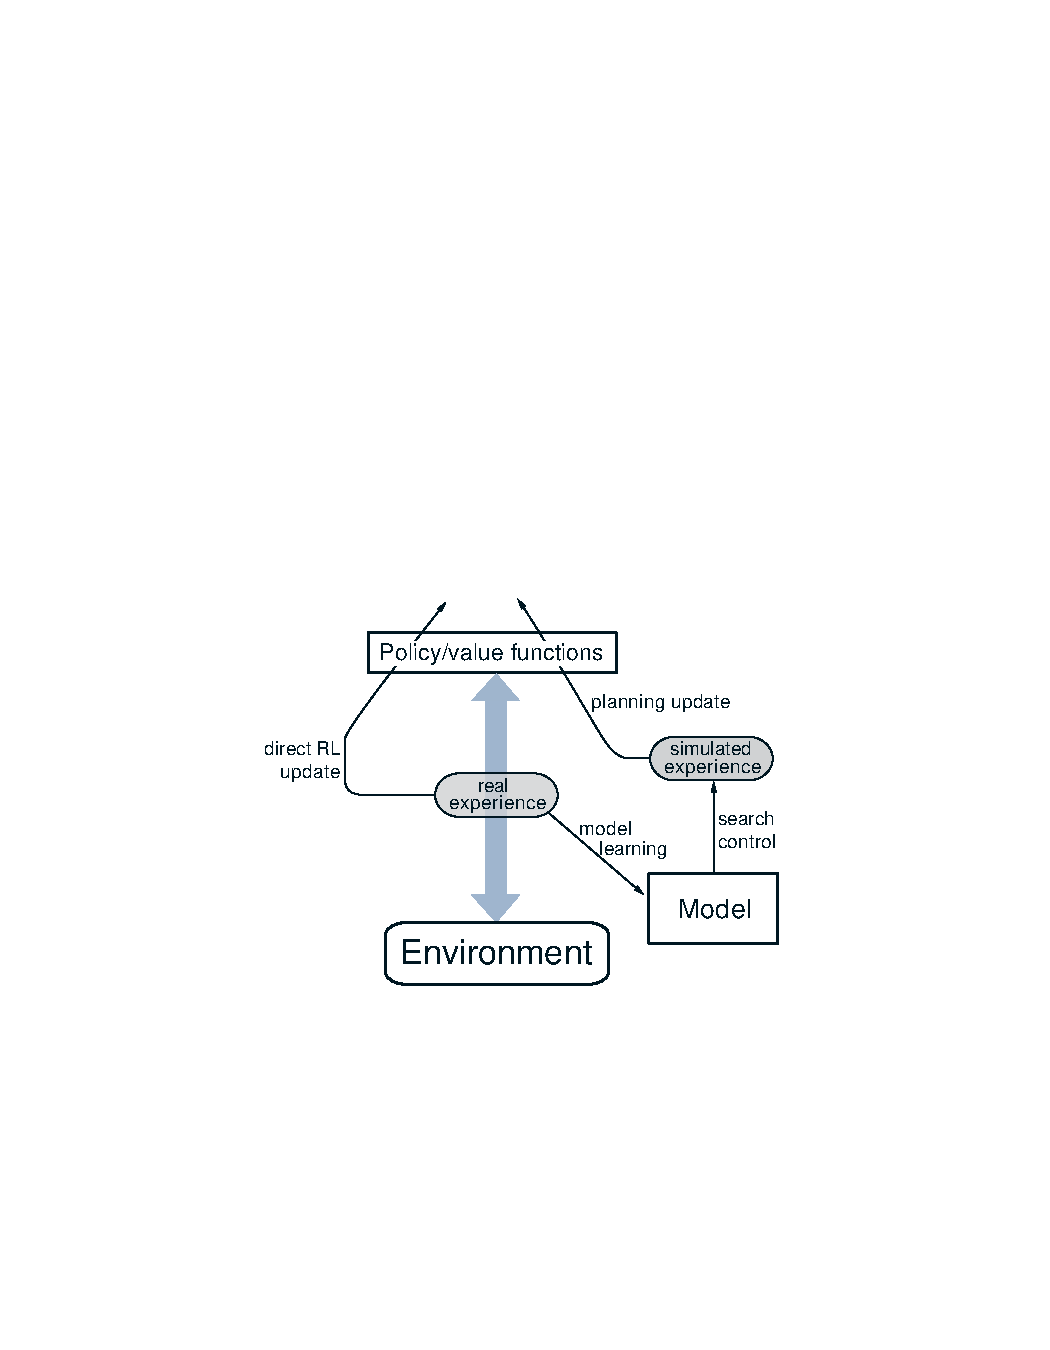
\includegraphics[width=7cm]{fig/lec07/Dyna.pdf}
	\caption{Dyna framework (source: R. Sutton and G. Barto, Reinforcement learning: an introduction, 2018, \href{https://creativecommons.org/licenses/by-nc-nd/2.0/}{CC BY-NC-ND 2.0})}
	\label{fig:Dyna}
\end{figure}
}

%%%%%%%%%%%%%%%%%%%%%%%%%%%%%%%%%%%%%%%%%%%%%%%%%%%%%%%%%%%%%
%% The General Dyna Architecture (2)%%
%%%%%%%%%%%%%%%%%%%%%%%%%%%%%%%%%%%%%%%%%%%%%%%%%%%%%%%%%%%%%
\frame{\frametitle{The General Dyna Architecture (2)}
\begin{itemize}
	\onslide<1->{\item \hl{Direct RL update}: any model-free algorithm: $Q$-learning, Sarsa, ...}
	\onslide<2->{\item \hl{Model learning}:
	\begin{itemize}
		\item In tabular case: simple distribution estimation as in \eqref{eq:dist_model}
		\item Simple experience buffer to re-apply model-free algorithm 
		\item For large or continuous state/action spaces: function approximation by supervised learning / system identification (next lecture)
	\end{itemize}}
	\onslide<3->{\item \hl{Search control}: strategies for selecting starting states and action to generate simulated experience}
\end{itemize}
\onslide<1->{\begin{figure}
	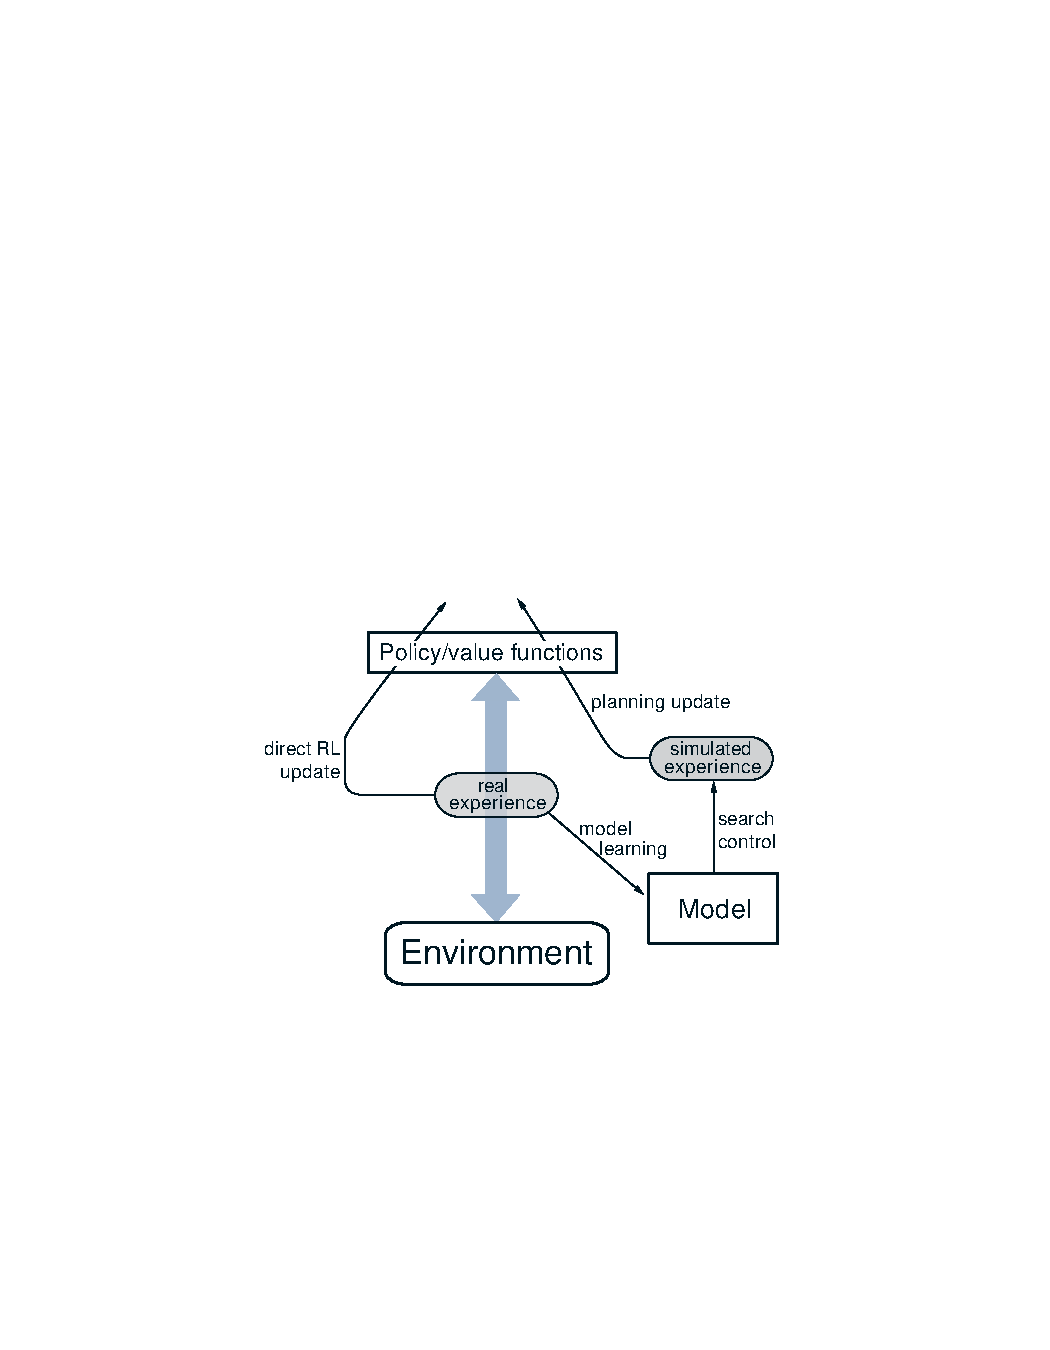
\includegraphics[width=5cm]{fig/lec07/Dyna.pdf}
\end{figure}}
}

%%%%%%%%%%%%%%%%%%%%%%%%%%%%%%%%%%%%%%%%%%%%%%%%%%%%%%%%%%%%%
%% Algorithmic Implementation: Dyna-Q %%
%%%%%%%%%%%%%%%%%%%%%%%%%%%%%%%%%%%%%%%%%%%%%%%%%%%%%%%%%%%%%
\frame{\frametitle{Algorithmic Implementation: Dyna-$Q$}

\setlength{\algomargin}{0.5em}
\begin{algorithm}[H]
\footnotesize
\SetKwInput{Input}{input} 
\SetKwInput{Output}{output}
\SetKwInput{Init}{init}
\SetKwInput{Param}{parameter}
\Param{$\alpha\in\left\{\mathbb{R}|0<\alpha<1\right\}, \quad n\in\left\{\mathbb{N}|n \geq 1\right\}$ (planning steps per real step)}
\Init{$\hat{q}(x,u)$ arbitrary (except terminal) and $\hat{\mathcal{M}}(x,u)$ $\forall \, \left\{x\in\mathcal{X}, u\in\mathcal{U}\right\}$}
\For{$j=1,2,\ldots$ episodes}{
	Initialize $x_0$\;
	$k \leftarrow 0$\;
	\Repeat{$x_k$ is terminal}{
				Choose $u_k$ from $x_k$ using a soft policy derived from $\hat{q}(x,u)$\;
				Take action $u_k$, observe $r_{k+1}$ and $x_{k+1}$\;
				$\hat{q}(x_k, u_k) \leftarrow \hat{q}(x_k, u_k) + \alpha\left[r_{k+1}+\gamma \max_{u} \hat{q}(x_{k+1}, u) - \hat{q}(x_k, u_k)\right]$\;
				$\hat{\mathcal{M}}(x_k,u_k)\leftarrow \left\{r_{k+1}, x_{k+1}\right\}$ (assuming deterministic env.)\;
				\For{$i=1,2,\ldots$ n}{
						$\tilde{x}_i\leftarrow$ random previously visited state\;
						$\tilde{u}_i\leftarrow$ random previously taken action in $\tilde{x}_i$\;
						$\left\{\tilde{r}_{i+1}, \tilde{x}_{i+1}\right\}\leftarrow\hat{\mathcal{M}}(\tilde{x}_i, \tilde{u}_i)$\;
						$\hat{q}(\tilde{x}_i, \tilde{u}_i) \leftarrow \hat{q}(\tilde{x}_i, \tilde{u}_i) + \alpha\left[\tilde{r}_{i+1}+\gamma \max_{u} \hat{q}(\tilde{x}_{i+1}, u) - \hat{q}(\tilde{x}_i, \tilde{u}_i)\right]$\;
				}
				$k \leftarrow k+1$\;
	}
}
\caption{Dyna with $Q$-learning (Dyna-$Q$)}
\label{algo:Dyna_Q}
\end{algorithm}
}

%%%%%%%%%%%%%%%%%%%%%%%%%%%%%%%%%%%%%%%%%%%%%%%%%%%%%%%%%%%%%
%% Remarks on Dyna-Q Implementation %%
%%%%%%%%%%%%%%%%%%%%%%%%%%%%%%%%%%%%%%%%%%%%%%%%%%%%%%%%%%%%%
\frame{\frametitle{Remarks on Dyna-$Q$ Implementation}
The specific Dyna-$Q$ characteristics are:
\begin{itemize}
	\item Direct RL update: $Q$-learning, 
	\item Model: simple memory buffer of previous real experience,
	\item Search strategy: random choices from model buffer.
\end{itemize}\pause
\vspace{0.5cm}
Moreover:
\begin{itemize}
	\item Number of Dyna planning steps $n$ is to be delimited from $n$-step bootstrapping (same symbol, two interpretations).\pause
	\item Without the model $\hat{\mathcal{M}}$ one would receive one-step $Q$-learning.\pause
	\item The model-based learning is done $n$ times per real environment interaction:
	\begin{itemize}
		\item Previous real experience is re-applied to $Q$-learning.
		\item Can be considered a \hl{background task}: choose $\max n$ s.t. hardware limitations (prevent turnaround errors).\pause 
	\end{itemize}  
	\item For stochastic environments: use a distributional model as in \eqref{eq:dist_model}.
	\begin{itemize}
		\item Update rule then may be modified from sample to expected update.
	\end{itemize}
\end{itemize}
}

%%%%%%%%%%%%%%%%%%%%%%%%%%%%%%%%%%%%%%%%%%%%%%%%%%%%%%%%%%%%%
%% Maze Example (1) %%
%%%%%%%%%%%%%%%%%%%%%%%%%%%%%%%%%%%%%%%%%%%%%%%%%%%%%%%%%%%%%
\frame{\frametitle{Maze Example (1)}
\begin{columns}[t,onlytextwidth]
\begin{column}{0.6\textwidth}
\begin{minipage}[c]{\linewidth}
\begin{figure}
	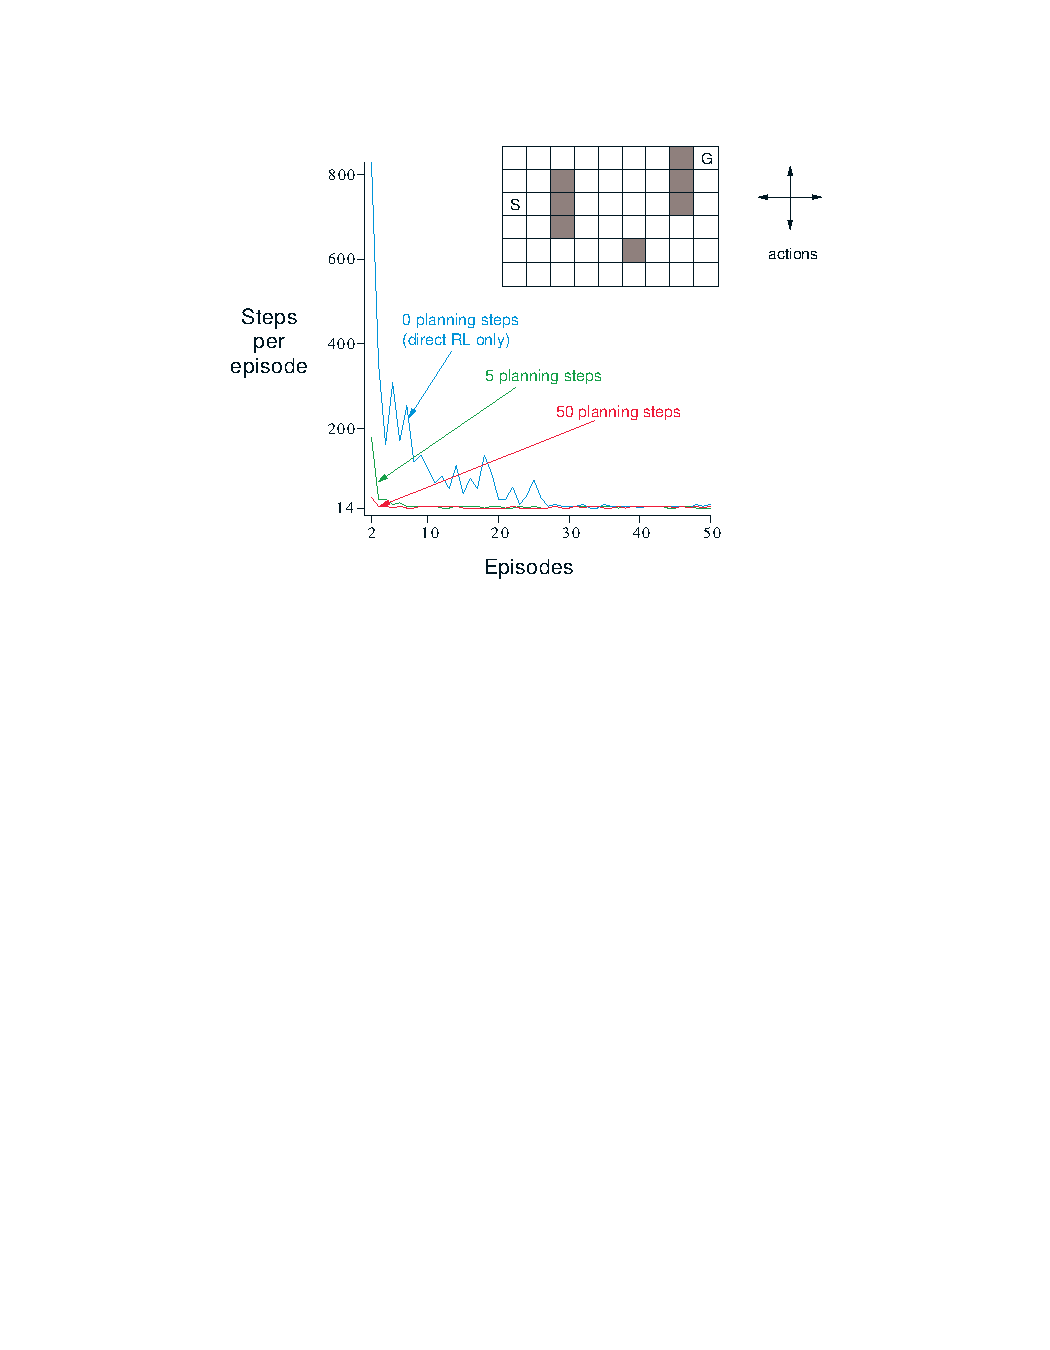
\includegraphics[width=7cm]{fig/lec07/Dyna_Simple_Maze.pdf}
	\caption{Applying Dyna-$Q$ with different planning steps $n$ to simple maze (source: R. Sutton and G. Barto, Reinforcement learning: an introduction, 2018, \href{https://creativecommons.org/licenses/by-nc-nd/2.0/}{CC BY-NC-ND 2.0})}
	\label{fig:Dyna_Simple_Maze}
\end{figure}
\end{minipage}
\end{column}
\hfill
\begin{column}{0.39\textwidth}
\begin{minipage}[c]{\linewidth}
	\begin{itemize}
		\item Maze with obstacles (gray blocks)
		\item Start at $S$ and reach $G$
		\item $r_T=+1$ at $G$
		\item Episodic task with $\gamma=0.95$
		\item Step size $\alpha=0.1$
		\item Exploration $\varepsilon=0.1$
		\item Averaged learning curves
	\end{itemize}
\end{minipage}
\end{column}
\end{columns}
}

%%%%%%%%%%%%%%%%%%%%%%%%%%%%%%%%%%%%%%%%%%%%%%%%%%%%%%%%%%%%%
%% Maze Example (2) %%
%%%%%%%%%%%%%%%%%%%%%%%%%%%%%%%%%%%%%%%%%%%%%%%%%%%%%%%%%%%%%
\frame{\frametitle{Maze Example (2)}
\begin{itemize}
	\item Blocks without an arrow depict a neutral policy (equal action values).
	\item Black squares indicate agent's position during second episode.
	\item Without planning ($n=0$), each episodes only adds one new item to the policy.
	\item With planning ($n=50$), the available experience is efficiently utilized.
		\item After the third episode, the planning agent found the optimal policy.
\end{itemize}
\begin{figure}
	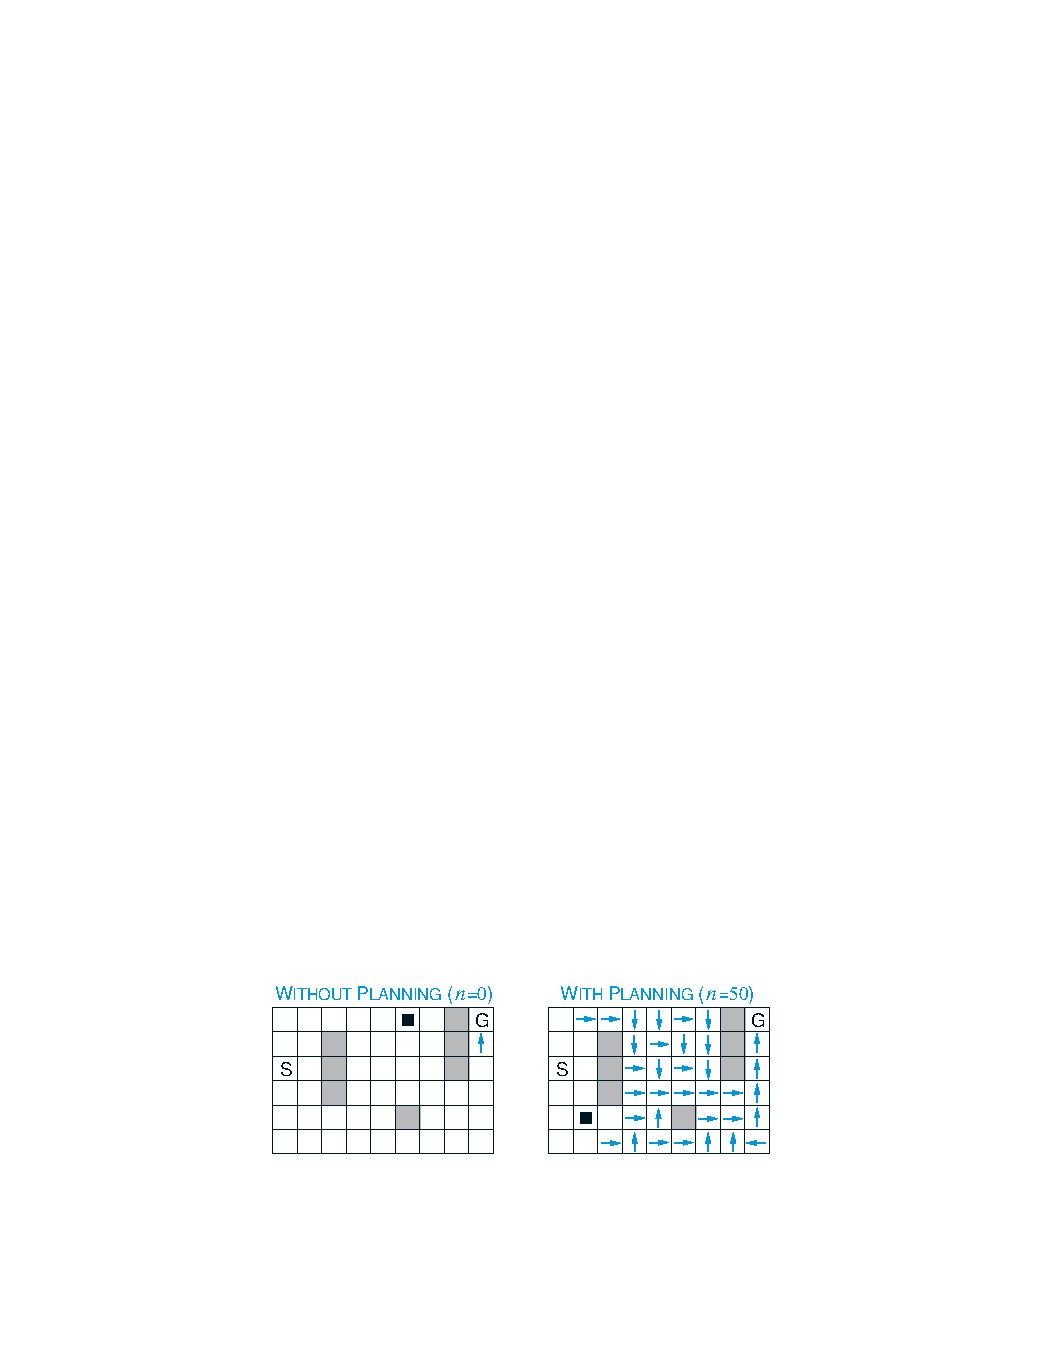
\includegraphics[width=7.5cm]{fig/lec07/Dyna_Simple_Maze_Updates.pdf}
	\caption{Policies (greedy action) for Dyna-$Q$ agent halfway through second episode (source: R. Sutton and G. Barto, Reinforcement learning: an introduction, 2018, \href{https://creativecommons.org/licenses/by-nc-nd/2.0/}{CC BY-NC-ND 2.0})}
	\label{fig:Dyna_Simple_Maze_Updates}
\end{figure}
}

%%%%%%%%%%%%%%%%%%%%%%%%%%%%%%%%%%%%%%%%%%%%%%%%%%%%%%%%%%%%%
%% What if the Model is Wrong? %%
%%%%%%%%%%%%%%%%%%%%%%%%%%%%%%%%%%%%%%%%%%%%%%%%%%%%%%%%%%%%%
\frame{\frametitle{What if the Model is Wrong?}
Possible model error sources:
\begin{itemize}
	\item A provided a priori model may be inaccurate (expert knowledge). \pause
	\item Environment behavior changes over time (non-stationary).\pause
	\item Early-stage model is biased due to learning process.\pause
	\item If function approximators are used: generalization error (cf. lecture 08 and following). \pause
\end{itemize}
\vspace{0.5cm}
Consequences:
\begin{itemize}
	\item Model errors are likely to lead to a suboptimal policy. \pause
	\item If lucky: errors are quickly discovered and directly corrected by default, random exploration.\pause
	\item Nevertheless, more intelligent exploration / correction strategies might be useful (compared to random actions as in $\varepsilon$-greedy strategies).
\end{itemize}
}

%%%%%%%%%%%%%%%%%%%%%%%%%%%%%%%%%%%%%%%%%%%%%%%%%%%%%%%%%%%%%
%% The Blocking Maze Example %%
%%%%%%%%%%%%%%%%%%%%%%%%%%%%%%%%%%%%%%%%%%%%%%%%%%%%%%%%%%%%%
\frame{\frametitle{The Blocking Maze Example}
\begin{columns}[t,onlytextwidth]
\begin{column}{0.6\textwidth}
\begin{minipage}[c]{\linewidth}
\begin{figure}
	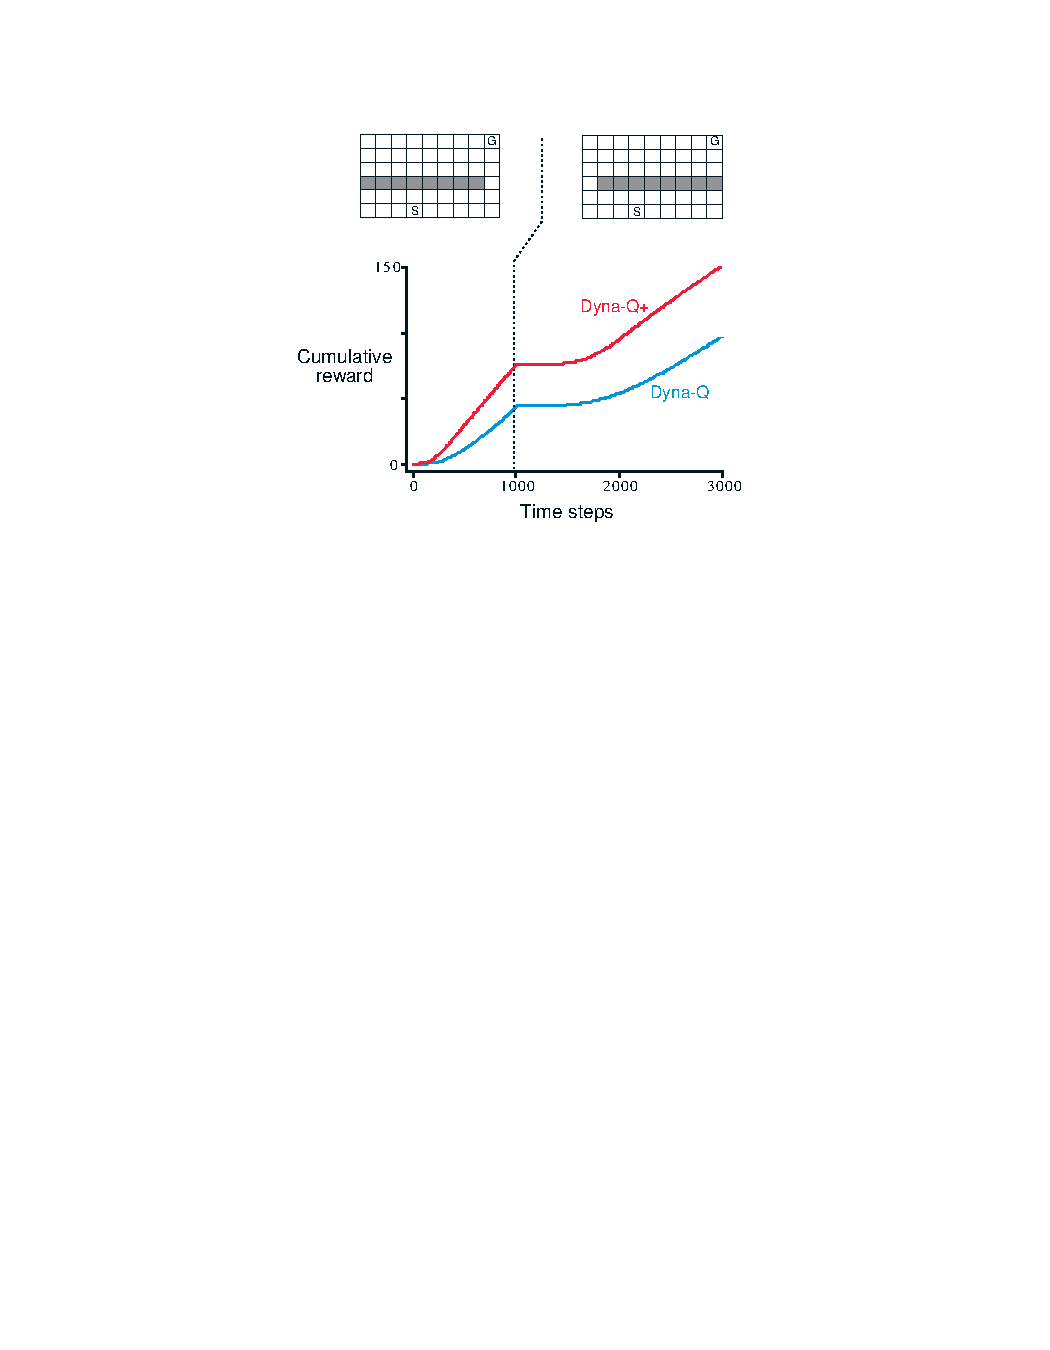
\includegraphics[width=6.75cm]{fig/lec07/Dyna_Q_Blocking.pdf}
	\caption{Maze with a changing layout after 1000 steps illustrates a model error (source: R. Sutton and G. Barto, Reinforcement learning: an introduction, 2018, \href{https://creativecommons.org/licenses/by-nc-nd/2.0/}{CC BY-NC-ND 2.0})}
	\label{fig:Dyna_Q_Blocking}
\end{figure}
\end{minipage}
\end{column}
\hfill
\begin{column}{0.39\textwidth}
\begin{minipage}[c]{\linewidth}
	\begin{itemize}
		\item Maze with a changing obstacle line
		\item Start at $S$ and reach $G$
		\item $r_T=+1$ at $G$
		\item Dyna-$Q+$ encourages intelligent exploration (upcoming slides)
		\item Dyna-$Q$ requires more steps in order to overcome the blockade
		\item Averaged learning curves
	\end{itemize}
\end{minipage}
\end{column}
\end{columns}
}

%%%%%%%%%%%%%%%%%%%%%%%%%%%%%%%%%%%%%%%%%%%%%%%%%%%%%%%%%%%%%
%% The Shortcut Maze Example %%
%%%%%%%%%%%%%%%%%%%%%%%%%%%%%%%%%%%%%%%%%%%%%%%%%%%%%%%%%%%%%
\frame{\frametitle{The Shortcut Maze Example}
\begin{columns}[t,onlytextwidth]
\begin{column}{0.6\textwidth}
\begin{minipage}[c]{\linewidth}
\begin{figure}
	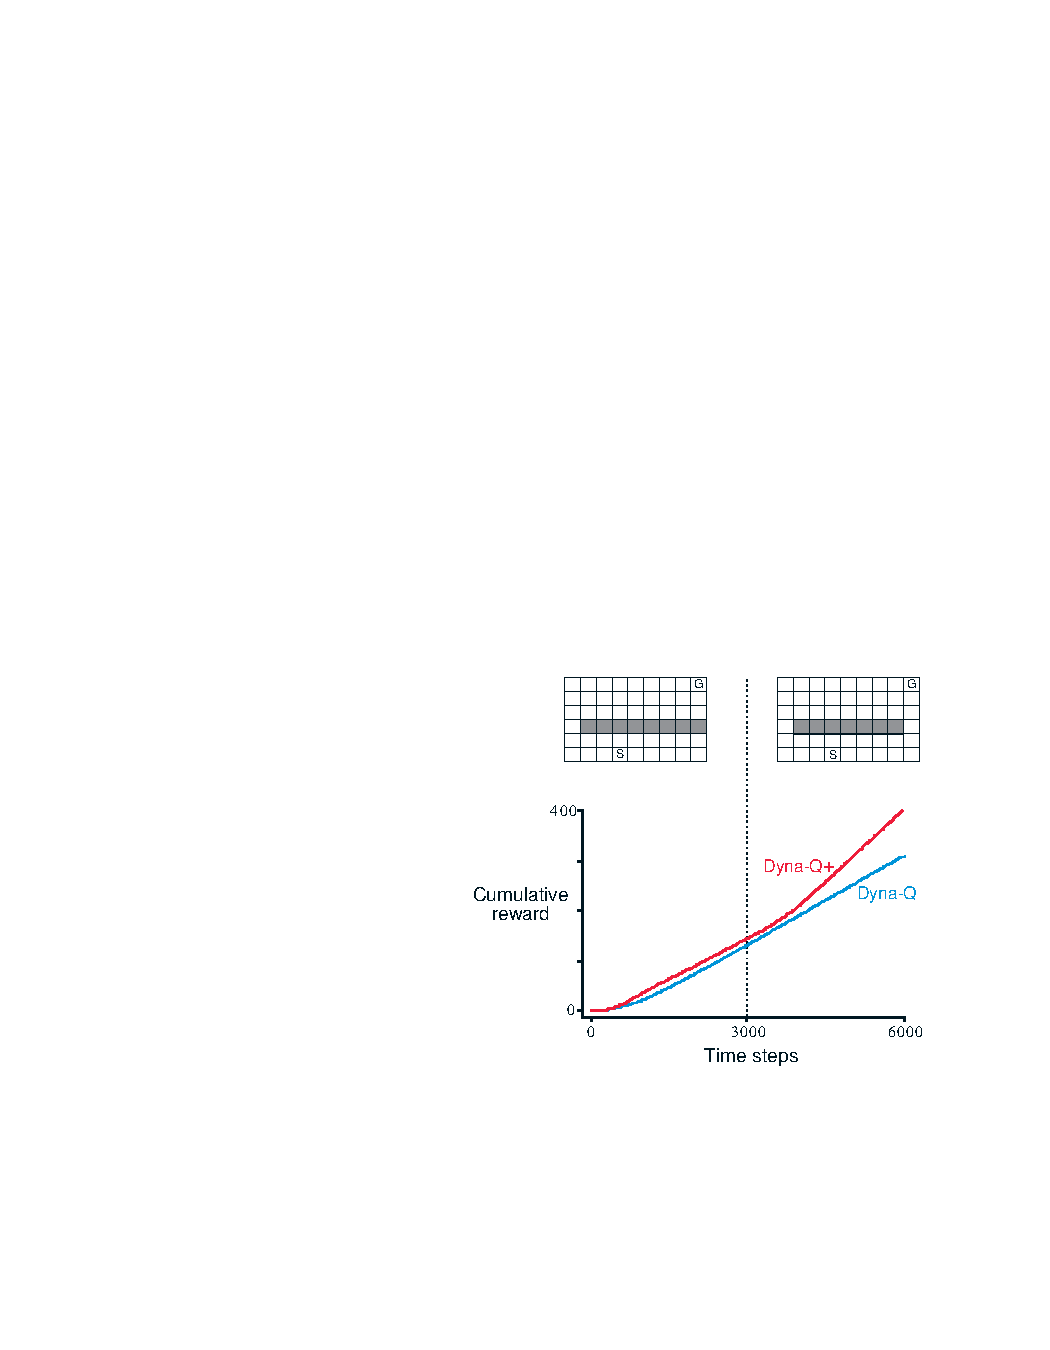
\includegraphics[width=6.75cm]{fig/lec07/Dyna_Q_Shortcut.pdf}
	\caption{Maze with an additional shortcut after 3000 steps (source: R. Sutton and G. Barto, Reinforcement learning: an introduction, 2018, \href{https://creativecommons.org/licenses/by-nc-nd/2.0/}{CC BY-NC-ND 2.0})}
	\label{fig:Dyna_Q_Shortcut}
\end{figure}
\end{minipage}
\end{column}
\hfill
\begin{column}{0.39\textwidth}
\begin{minipage}[c]{\linewidth}
	\begin{itemize}
		\item Maze opens a shortcut after 3000 steps
		\item Start at $S$ and reach $G$
		\item $r_T=+1$ at $G$
		\item Dyna-$Q$ with random exploration is likely not finding the shortcut
		\item Dyna-$Q$+ exploration strategy is able to correct internal model
		\item Averaged learning curves
	\end{itemize}
\end{minipage}
\end{column}
\end{columns}
}

%%%%%%%%%%%%%%%%%%%%%%%%%%%%%%%%%%%%%%%%%%%%%%%%%%%%%%%%%%%%%
%% Dyna-Q+ Extensions %%
%%%%%%%%%%%%%%%%%%%%%%%%%%%%%%%%%%%%%%%%%%%%%%%%%%%%%%%%%%%%%
\frame{\frametitle{Dyna-$Q$+ Extensions}
Compared to default Dyna-$Q$ in \algoref{algo:Dyna_Q}, Dyna-$Q$+ contains the following extensions: 
\begin{itemize}
	\item Search heuristic: add $\kappa \sqrt{\tau}$ to regular reward.
	\begin{itemize}
		\item $\tau$: is the number of time steps a state-action transition has not been tried.
		\item $\kappa$: is a small scaling factor $\kappa\in\left\{\mathbb{R}|0<\kappa\right\}$.
		\item Agent is encouraged to keep testing all accessible transitions.
	\end{itemize}\pause
	\vspace{0.25cm}
	\item Actions for given states that had never been tried before are allowed for simulation-based planning.
	\begin{itemize}
		\item Initial model for that: actions lead back to same state without reward.
	\end{itemize}
\end{itemize}
}

%%%%%%%%%%%%%%%%%%%%%%%%%%%%%%%%%%%%%%%%%%%%%%%%%%%%%%%%%%%%%%%%%%
\section{Prioritized Sweeping} 
%%%%%%%%%%%%%%%%%%%%%%%%%%%%%%%%%%%%%%%%%%%%%%%%%%%%%%%%%%%%%%%%%%
\begin{frame}
\frametitle{Table of Contents}
\tableofcontents[currentsection]
\end{frame}

%%%%%%%%%%%%%%%%%%%%%%%%%%%%%%%%%%%%%%%%%%%%%%%%%%%%%%%%%%%%%
%% Background and Idea %%
%%%%%%%%%%%%%%%%%%%%%%%%%%%%%%%%%%%%%%%%%%%%%%%%%%%%%%%%%%%%%
\frame{\frametitle{Background and Idea}

\begin{itemize}
	\item Dyna-$Q$ randomly samples from the memory buffer.
	\begin{itemize}
		\item Many planning updates maybe pointless, e.g., zero-valued state updates during early training.
		\item In large state-action spaces: inefficient search since transitions are chosen far away from optimal policies. 
	\end{itemize}\pause
	\vspace{0.5cm}
	\item Better: focus on important updates.
	\begin{itemize}
		\item In episodic tasks: \hl{backward focusing} starting from the goal state.
		\item In continuing tasks: \hl{prioritize} according to impact on value updates. \pause
	\end{itemize}
	\vspace{0.5cm}
	\item Solution method is called \hl{prioritized sweeping}.
	\begin{itemize}
		\item Build up a queue of every state-action pair whose value would change significantly. 
		\item Prioritize updates by the size of change.
		\item Neglect state-action pairs with only minor impact.
	\end{itemize}
\end{itemize}
}

%%%%%%%%%%%%%%%%%%%%%%%%%%%%%%%%%%%%%%%%%%%%%%%%%%%%%%%%%%%%%
%% Algorithmic Implementation: Prioritized sweeping %%
%%%%%%%%%%%%%%%%%%%%%%%%%%%%%%%%%%%%%%%%%%%%%%%%%%%%%%%%%%%%%
\frame{\frametitle{Algorithmic Implementation: Prioritized Sweeping}
\vspace{-0.15cm}
\setlength{\algomargin}{0.5em}
\begin{algorithm}[H]
\footnotesize
\SetKwInput{Input}{input} 
\SetKwInput{Output}{output}
\SetKwInput{Init}{init}
\SetKwInput{Param}{parameter}
\Param{$\alpha\in\left\{\mathbb{R}|0<\alpha<1\right\}, \quad n\in\left\{\mathbb{N}|n \geq 1\right\}, \quad \theta\in\left\{\mathbb{R}|\theta \geq 0\right\}$}
\Init{$\hat{q}(x,u)$ arbitrary and $\hat{\mathcal{M}}(x,u)$ $\forall \, \left\{x\in\mathcal{X}, u\in\mathcal{U}\right\}$, empty queue $\mathcal{Q}$}
\For{$j=1,2,\ldots$ episodes}{
	Initialize $x_0$ and $k \leftarrow 0$\;
	\Repeat{$x_k$ is terminal}{
				Choose $u_k$ from $x_k$ using a soft policy derived from $\hat{q}(x,u)$\;
				Take action $u_k$, observe $r_{k+1}$ and $x_{k+1}$\;
				%$\hat{q}(x_k, u_k) \leftarrow \hat{q}(x_k, u_k) + \alpha\left[r_{k+1}+\gamma \max_{u} \hat{q}(x_{k+1}, u) - \hat{q}(x_k, u_k)\right]$\;
				$\hat{\mathcal{M}}(x_k,u_k)\leftarrow \left\{r_{k+1}, x_{k+1}\right\}$ (assuming deterministic env.)\;
				$P \leftarrow \left|r_{k+1}+\gamma \max_{u} \hat{q}(x_{k+1}, u) - \hat{q}(x_k, u_k)\right|$\;
				\lIf{$P>\theta$}{insert $\left\{x_{k}, u_{k}\right\}$ in $\mathcal{Q}$ with priority $P$}
				\For{$i=1,2,\ldots$ n while queue $\mathcal{Q}$ is not empty}{
						$\left\{\tilde{x}_{i}, \tilde{u}_{i}\right\}\leftarrow \argmax_{P}(\mathcal{Q})$\;
						$\left\{\tilde{r}_{i+1}, \tilde{x}_{i+1}\right\}\leftarrow\hat{\mathcal{M}}(\tilde{x}_i, \tilde{u}_i)$\;
						$\hat{q}(\tilde{x}_i, \tilde{u}_i) \leftarrow \hat{q}(\tilde{x}_i, \tilde{u}_i) + \alpha\left[\tilde{r}_{i+1}+\gamma \max_{u} \hat{q}(\tilde{x}_{i+1}, u) - \hat{q}(\tilde{x}_i, \tilde{u}_i)\right]$\;
						\For{$\forall \left\{\overline{x}, \overline{u}\right\}$ predicted to lead to $\tilde{x}_i$}{
						$\overline{r}\leftarrow$ predicted reward for $\left\{\overline{x}, \overline{u}, \tilde{x}_i\right\}$\;
						$P \leftarrow \left|\overline{r}+\gamma \max_{u} \hat{q}(\tilde{x}_i, u) - \hat{q}(\overline{x}, \overline{u})\right|$\;
						\lIf{$P>\theta$}{insert $\left\{\overline{x}, \overline{u}\right\}$ in $\mathcal{Q}$ with priority $P$}
						}
				}
				$k \leftarrow k+1$\;
	}
}
%\caption{Prioritized sweeping}
\label{algo:prior_sweeping}
\end{algorithm}
}

%%%%%%%%%%%%%%%%%%%%%%%%%%%%%%%%%%%%%%%%%%%%%%%%%%%%%%%%%%%%%
%% Remarks on Prioritized Sweeping Implementation %%
%%%%%%%%%%%%%%%%%%%%%%%%%%%%%%%%%%%%%%%%%%%%%%%%%%%%%%%%%%%%%
\frame{\frametitle{Remarks on Prioritized Sweeping Implementation}
The specific prioritized sweeping characteristics are:
\begin{itemize}
	\item Direct RL update: $Q$-learning, 
	\item Model: simple memory buffer of previous real experience,
	\item \hl{Search strategy}: prioritized updates based on predicted value change.
\end{itemize}\pause
\vspace{0.5cm}
Moreover:
\begin{itemize}
	\item $\theta$ is a hyperparameter denoting the update significance threshold.\pause
	\item Prediction step regarding $\tilde{x}_i$ is a backward search in the model buffer.\pause
	\item For stochastic environments: use a distributional model as in \eqref{eq:dist_model}.
	\begin{itemize}
		\item Update rule then may be modified from sample to expected update.
	\end{itemize}
\end{itemize}
}

%%%%%%%%%%%%%%%%%%%%%%%%%%%%%%%%%%%%%%%%%%%%%%%%%%%%%%%%%%%%%
%% Comparing Against Dyna-$Q$ on Simple Maze Example %%
%%%%%%%%%%%%%%%%%%%%%%%%%%%%%%%%%%%%%%%%%%%%%%%%%%%%%%%%%%%%%
\frame{\frametitle{Comparing Against Dyna-$Q$ on Simple Maze Example}
\begin{columns}[t,onlytextwidth]
\begin{column}{0.6\textwidth}
\begin{minipage}[c]{\linewidth}
\begin{figure}
	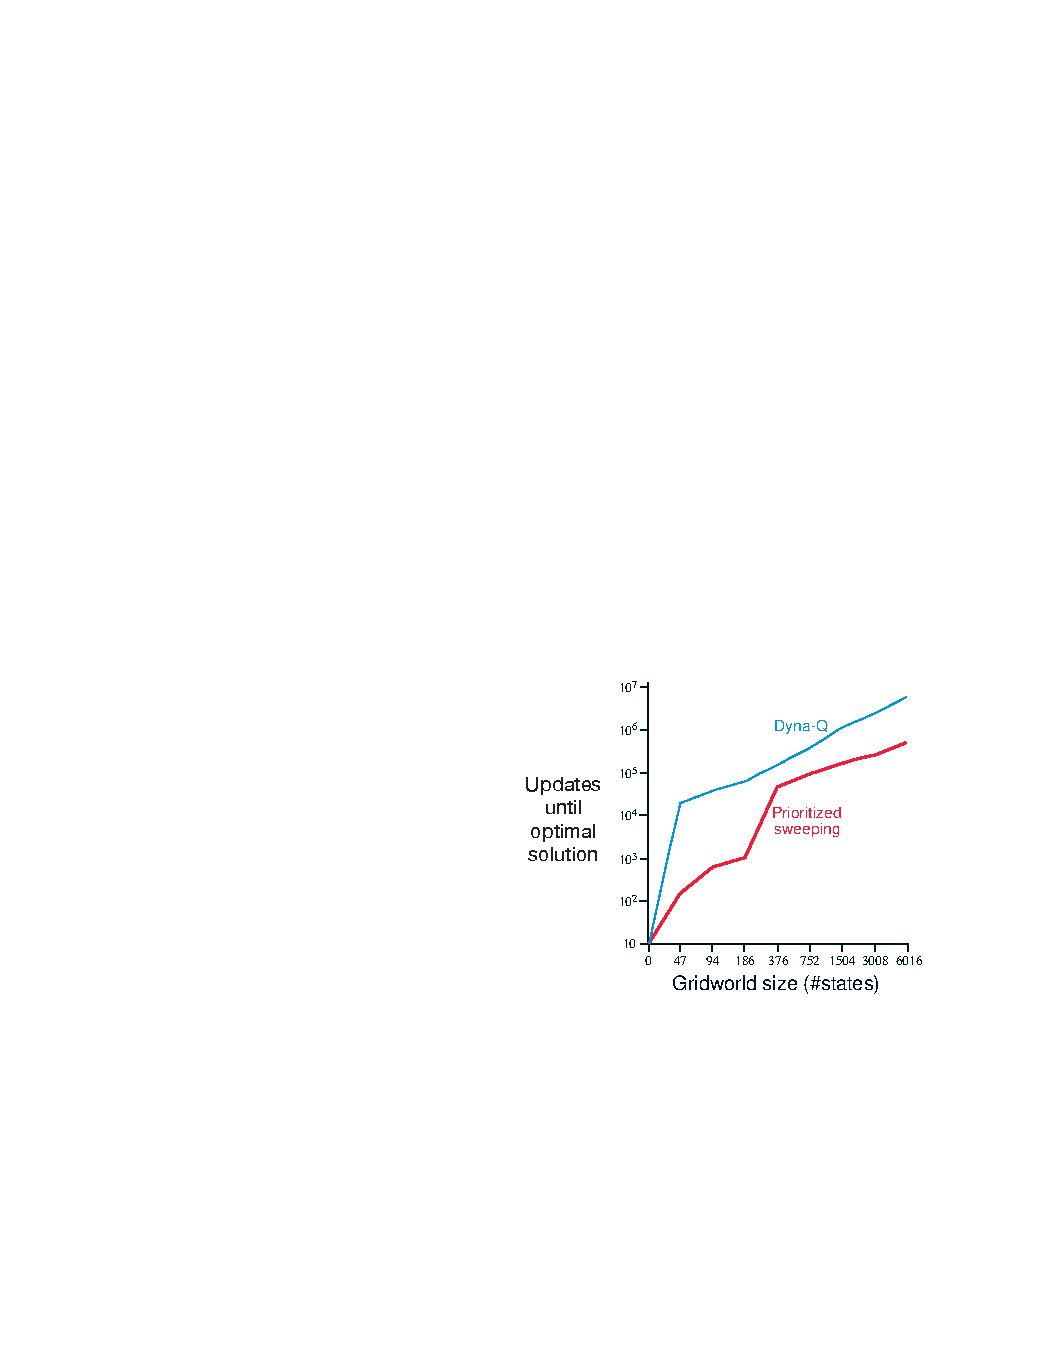
\includegraphics[width=6.75cm]{fig/lec07/Prior_Sweeping_Dyna.pdf}
	\caption{Comparison of prioritized sweeping and Dyna-$Q$ on simple maze (source: R. Sutton and G. Barto, Reinforcement learning: an introduction, 2018, \href{https://creativecommons.org/licenses/by-nc-nd/2.0/}{CC BY-NC-ND 2.0})}
	\label{fig:Prior_Sweeping_Dyna}
\end{figure}
\end{minipage}
\end{column}
\hfill
\begin{column}{0.39\textwidth}
\begin{minipage}[c]{\linewidth}
	\begin{itemize}
		\item Environment framework as in \figref{fig:Dyna_Simple_Maze}
		\item But: changing maze sizes (number of states)
		\item Both methods can utilize up to $n=5$ planning steps
		\item Prioritized sweeping finds optimal solution 5-10 times quicker
	\end{itemize}
\end{minipage}
\end{column}
\end{columns}
}

%%%%%%%%%%%%%%%%%%%%%%%%%%%%%%%%%%%%%%%%%%%%%%%%%%%%%%%%%%%%%%%%%%
\section{Update Variants} 
%%%%%%%%%%%%%%%%%%%%%%%%%%%%%%%%%%%%%%%%%%%%%%%%%%%%%%%%%%%%%%%%%%
\begin{frame}
\frametitle{Table of Contents}
\tableofcontents[currentsection]
\end{frame}

%%%%%%%%%%%%%%%%%%%%%%%%%%%%%%%%%%%%%%%%%%%%%%%%%%%%%%%%%%%%%
%% Update Rule Alternatives %%
%%%%%%%%%%%%%%%%%%%%%%%%%%%%%%%%%%%%%%%%%%%%%%%%%%%%%%%%%%%%%
\frame{\frametitle{Update Rule Alternatives}
\begin{itemize}
	\item Dyna updates (search strategy) are not bound to $Q$-learning during planning and can be exchanged in many ways (see \figref{fig:Backup_one_step}).
	\item Even evaluating a fixed policy $\pi$ in terms of $v_\pi(x)$ and $q_\pi(x,u)$ is possible.
\end{itemize}
\begin{figure}
	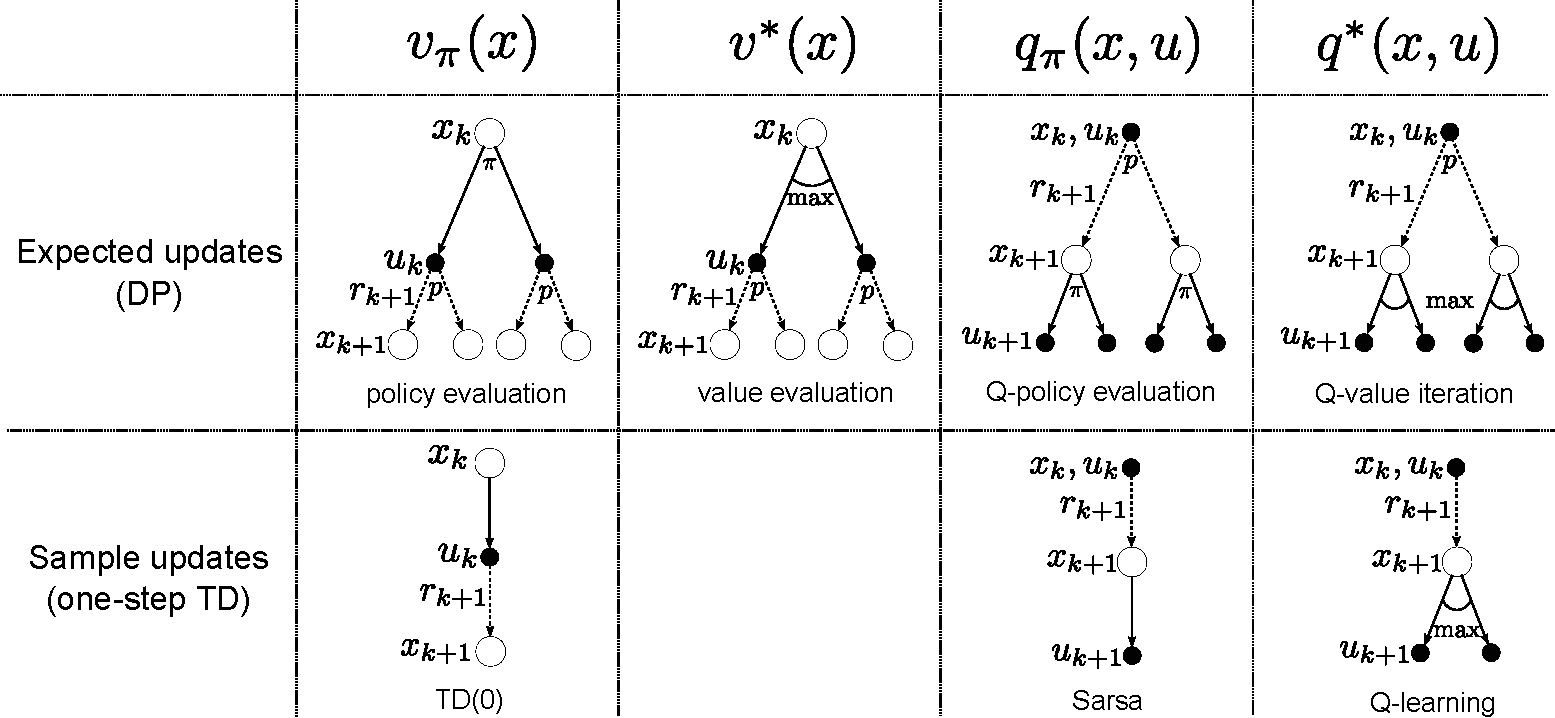
\includegraphics[width=11cm]{fig/lec07/Backup_one_step.pdf}
	\caption{Possible one-step updates: alternatives for Dyna}
	\label{fig:Backup_one_step}
\end{figure}
}

%%%%%%%%%%%%%%%%%%%%%%%%%%%%%%%%%%%%%%%%%%%%%%%%%%%%%%%%%%%%%
%% Advantages and Drawbacks: Expected vs. Sampled Updates %%
%%%%%%%%%%%%%%%%%%%%%%%%%%%%%%%%%%%%%%%%%%%%%%%%%%%%%%%%%%%%%
\frame{\frametitle{Advantages \& Drawbacks: Expected vs. Sampled Updates}
Pro expected updates:
\begin{itemize}
	\item Delivers more accurate value estimates (no sampling error).  \pause
\end{itemize}
\vspace{0.25cm}
Pro sample updates:
\begin{itemize}
	\item Is computational cheaper (e.g., distributional model not required). \pause
\end{itemize}
\vspace{0.25cm}
Leads to trade-off:
\begin{itemize}
	\item Estimation accuracy vs. computational burden.\pause
	\item Evaluate decision on given problem, i.e., how many state-action pairs have to be evaluated for a new expected update?\pause
	\item Utilize \hl{branching factor $b$} metric: corresponds to number of possible next states $x'$ with $p(x'|x,u)>0$. 
	\begin{itemize}
		\item If expected update is available, this will be roughly as accurate as $b$ samplings.
		\item If only incomplete expected update is available, prefer sampling solution (often applies to large state-action spaces).
	\end{itemize}
\end{itemize}
}

%%%%%%%%%%%%%%%%%%%%%%%%%%%%%%%%%%%%%%%%%%%%%%%%%%%%%%%%%%%%%
%% Example for Sampled vs. Expected Updates %%
%%%%%%%%%%%%%%%%%%%%%%%%%%%%%%%%%%%%%%%%%%%%%%%%%%%%%%%%%%%%%
\frame{\frametitle{Example for Sampled vs. Expected Updates}
\begin{itemize}
	\item Artificial prediction task where all $b$ successor states are equally likely
	\item Method initialization such that RMS error is always one 
	\item Sample updates perform particularly well for large branching factors $b$ (takeaway message: \hl{if facing large stochastic problems, use sampling})
\end{itemize}
\begin{figure}
	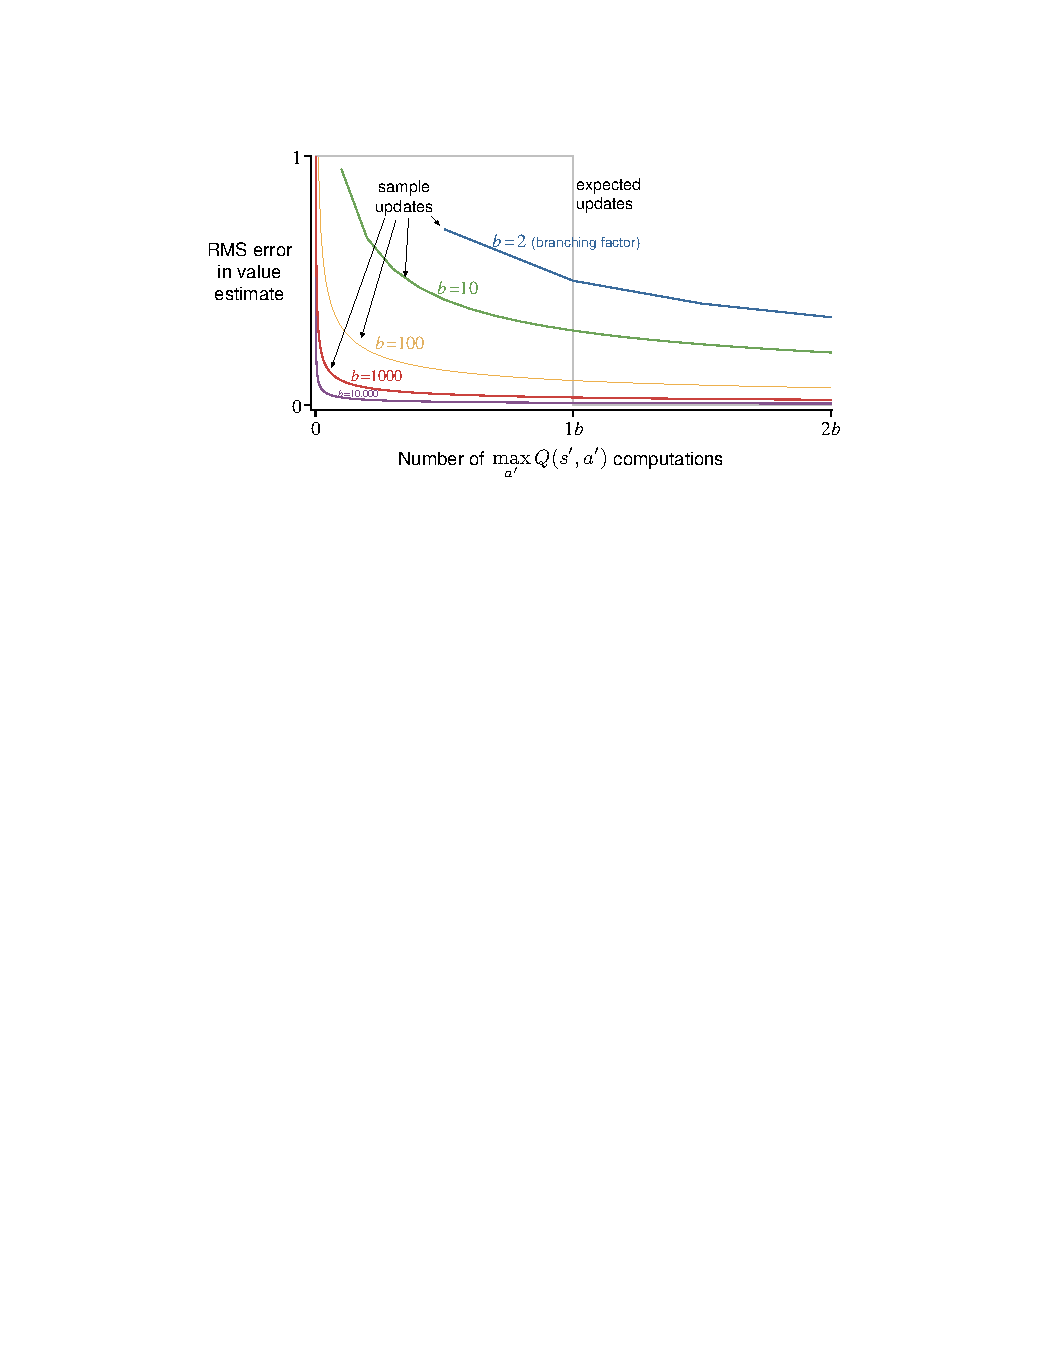
\includegraphics[width=8.5cm]{fig/lec07/Expected_vs_sample_updates_example.pdf}
	\caption{Comparison of expected vs. sampled updates (source: R. Sutton and G. Barto, Reinforcement learning: an introduction, 2018, \href{https://creativecommons.org/licenses/by-nc-nd/2.0/}{CC BY-NC-ND 2.0})}
	\label{fig:Expected_vs_sample_updates_example}
\end{figure}
}

%%%%%%%%%%%%%%%%%%%%%%%%%%%%%%%%%%%%%%%%%%%%%%%%%%%%%%%%%%%%%
%% Alternative on Distributing the Updates %%
%%%%%%%%%%%%%%%%%%%%%%%%%%%%%%%%%%%%%%%%%%%%%%%%%%%%%%%%%%%%%
\frame{\frametitle{Alternatives on Distributing the Updates}
Recap:
\begin{itemize}
	\item Dynamic programming: sweep through the entire state(-action) space
	\item Dyna-$Q$: random uniform sampling
	\item Mutual problem: irrelevant updates decrease computational efficiency
\end{itemize}\pause
\vspace{0.5cm}
Alternative: update according to on-policy distribution
\begin{itemize}
	\item Based on sampling along the encountered state(-action) pairs (\hl{trajectory sweeping})\pause
	\item Based on explicit on-policy distribution\pause
	\item In both cases: ignore vast, uninteresting parts of the problem space at the risk of updating same old parts all over again 
\end{itemize}
}

%%%%%%%%%%%%%%%%%%%%%%%%%%%%%%%%%%%%%%%%%%%%%%%%%%%%%%%%%%%%%
%% Exemplary Update Distribution Comparison %%
%%%%%%%%%%%%%%%%%%%%%%%%%%%%%%%%%%%%%%%%%%%%%%%%%%%%%%%%%%%%%
\frame{\frametitle{Exemplary Update Distribution Comparison}
\begin{columns}[t,onlytextwidth]
\begin{column}{0.62\textwidth}
\begin{minipage}[c]{\linewidth}
\begin{figure}
	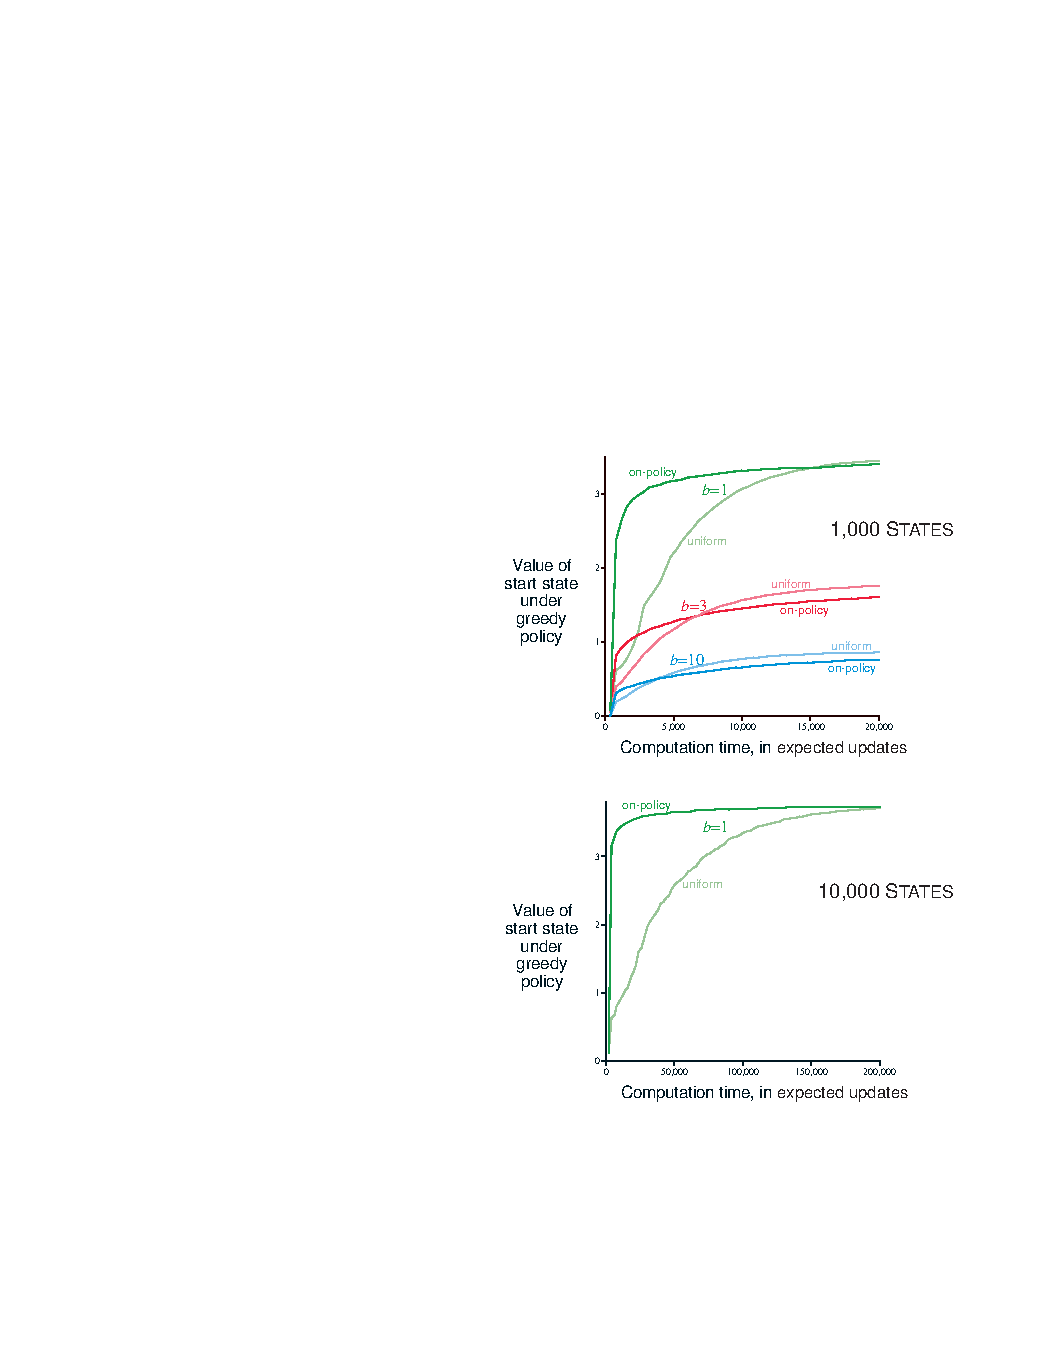
\includegraphics[width=4.5cm]{fig/lec07/Trajectory_sampling.pdf}
	\caption{Update distribution comparison (source: R. Sutton and G. Barto, Reinforcement learning: an introduction, 2018, \href{https://creativecommons.org/licenses/by-nc-nd/2.0/}{CC BY-NC-ND 2.0})}
	\label{fig:Trajectory_sampling}
\end{figure}
\end{minipage}
\end{column}
\hfill
\begin{column}{0.39\textwidth}
\begin{minipage}[c]{\linewidth}
Example:
	\begin{itemize}
		\item Two actions per state
		\item Both actions led to $b$ next states
		\item $10\,\%$ probability of transition to terminal state
		\item reward per transition: $\mathcal{N}(\mu=0, \sigma^2=1)$
		\item Task: estimate start state value
		\item 200 randomly generated undiscounted episodic runs
	\end{itemize}
\end{minipage}
\end{column}
\end{columns}
}

%%%%%%%%%%%%%%%%%%%%%%%%%%%%%%%%%%%%%%%%%%%%%%%%%%%%%%%%%%%%%%%%%%
\section{Planning at Decision Time} 
%%%%%%%%%%%%%%%%%%%%%%%%%%%%%%%%%%%%%%%%%%%%%%%%%%%%%%%%%%%%%%%%%%
\begin{frame}
\frametitle{Table of Contents}
\tableofcontents[currentsection]
\end{frame}

%%%%%%%%%%%%%%%%%%%%%%%%%%%%%%%%%%%%%%%%%%%%%%%%%%%%%%%%%%%%%
%% Background Planning vs. Planning at Decision Time %%
%%%%%%%%%%%%%%%%%%%%%%%%%%%%%%%%%%%%%%%%%%%%%%%%%%%%%%%%%%%%%
\frame{\frametitle{Background Planning vs. Planning at Decision Time}
\hl{Background Planning} (discussed so far):
\begin{itemize}
	\item Gradually improves policy or value function if time is available.
	\item Backward view: re-apply gathered experience. \pause
	\item Feasible for fast execution: policy or value estimate are available with low latency (important, e.g., for real-time control). \pause
\end{itemize}
\vspace{0.5cm}
\hl{Planning at decision time}\footnote[1]{\onslide<3->{Can be interpreted as \textit{model predictive control} in an engineering context.}} (not yet discussed alternative):
\begin{itemize}
	\item Select single next future action through planning.
	\item Forward view: predict future trajectories starting from current state. \pause
	\item Typically discards previous planning outcomes (start from scratch after state transition).\pause
	\item If multiple trajectories are independent: easy parallel implementation.\pause
	\item Most useful if fast responses are not required (e.g., turn-based games).
\end{itemize}
}

%%%%%%%%%%%%%%%%%%%%%%%%%%%%%%%%%%%%%%%%%%%%%%%%%%%%%%%%%%%%%
%% Heuristic Search %%
%%%%%%%%%%%%%%%%%%%%%%%%%%%%%%%%%%%%%%%%%%%%%%%%%%%%%%%%%%%%%
\frame{\frametitle{Heuristic Search}
\begin{itemize}
	\item Develop \hl{tree-like continuations} from each state encountered. 
	\item Approximate value function at leaf nodes (using a model) and back up towards the current state.
	\item Choose action according to predicted trajectory with highest value. 
	\item Predictions are normally discarded (new search tree in each state). 
\end{itemize}
\begin{figure}
	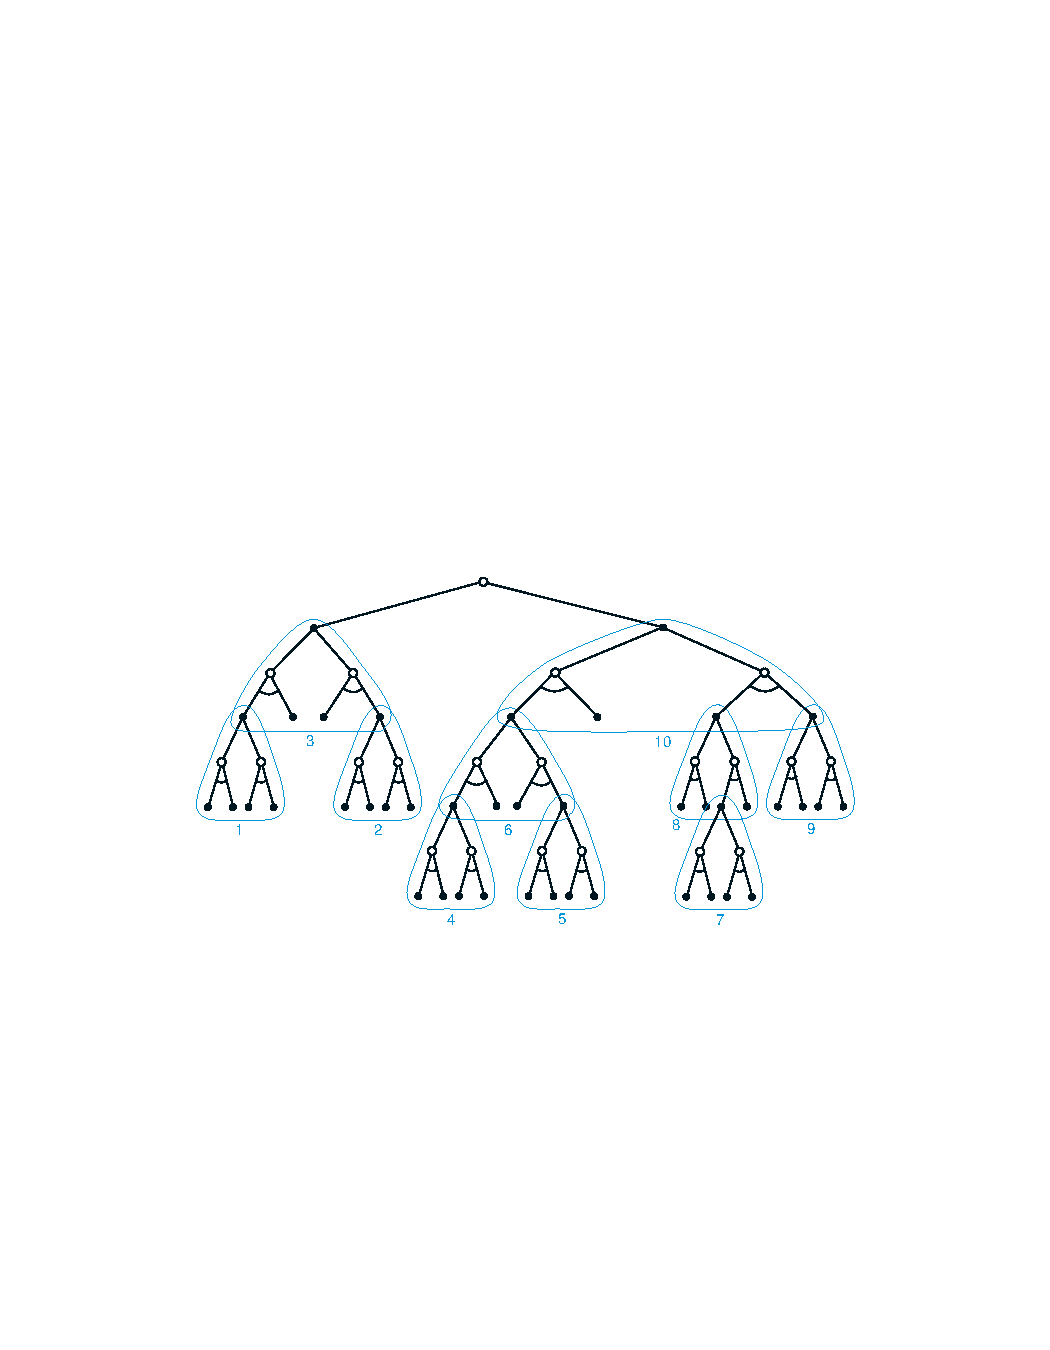
\includegraphics[width=7.0cm]{fig/lec07/Heuristic_search_tree.pdf}
	\caption{Heuristic search tree with exemplary order of back-up operations (source: R. Sutton and G. Barto, Reinforcement learning: an introduction, 2018, \href{https://creativecommons.org/licenses/by-nc-nd/2.0/}{CC BY-NC-ND 2.0})}
	\label{fig:Heuristic_search_tree}
\end{figure}
}

%%%%%%%%%%%%%%%%%%%%%%%%%%%%%%%%%%%%%%%%%%%%%%%%%%%%%%%%%%%%%
%% Rollout Algorithms %%
%%%%%%%%%%%%%%%%%%%%%%%%%%%%%%%%%%%%%%%%%%%%%%%%%%%%%%%%%%%%%
\frame{\frametitle{Rollout Algorithms}
\begin{itemize}
	\item Similar to heuristic search, but: \hl{simulate trajectories following a rollout policy}.
	\item Use Monte Carlo estimates of action value \hl{only for current state} to evaluate on best action.
	\item Gradually improves rollout policy but optimal policy might not be found if rollout sequences are too short. 
	\item Predictions are normally discarded (new rollout in each state). 
\end{itemize}
\begin{figure}
	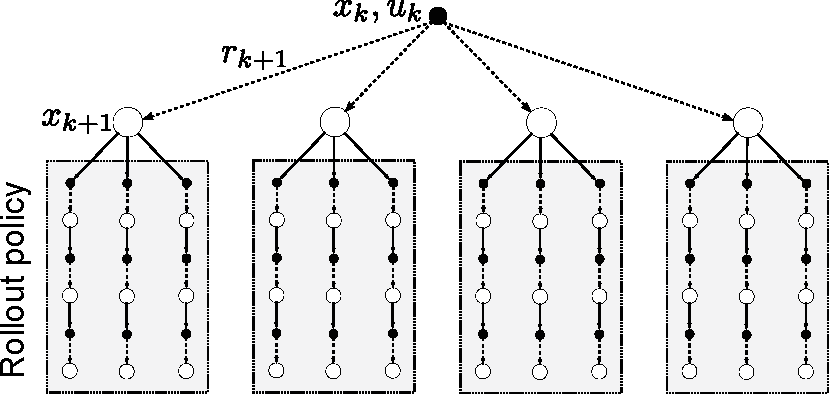
\includegraphics[width=6.5cm]{fig/lec07/Rollout.pdf}
	\caption{Simplified processing diagram of rollout algorithms}
	\label{fig:Rollout}
\end{figure}
}

%%%%%%%%%%%%%%%%%%%%%%%%%%%%%%%%%%%%%%%%%%%%%%%%%%%%%%%%%%%%%
%% Monte Carlo Tree Search (MCTS) %%
%%%%%%%%%%%%%%%%%%%%%%%%%%%%%%%%%%%%%%%%%%%%%%%%%%%%%%%%%%%%%
\frame{\frametitle{Monte Carlo Tree Search (MCTS)}
\begin{itemize}
	\item Rollout algorithm, but: 
	\begin{itemize}
		\item \hl{accumulates values estimates} from former MC simulations,
		\item makes use of an \hl{informed tree policy} (e.g., $\varepsilon$-greedy).
	\end{itemize}
\end{itemize}
\begin{figure}
	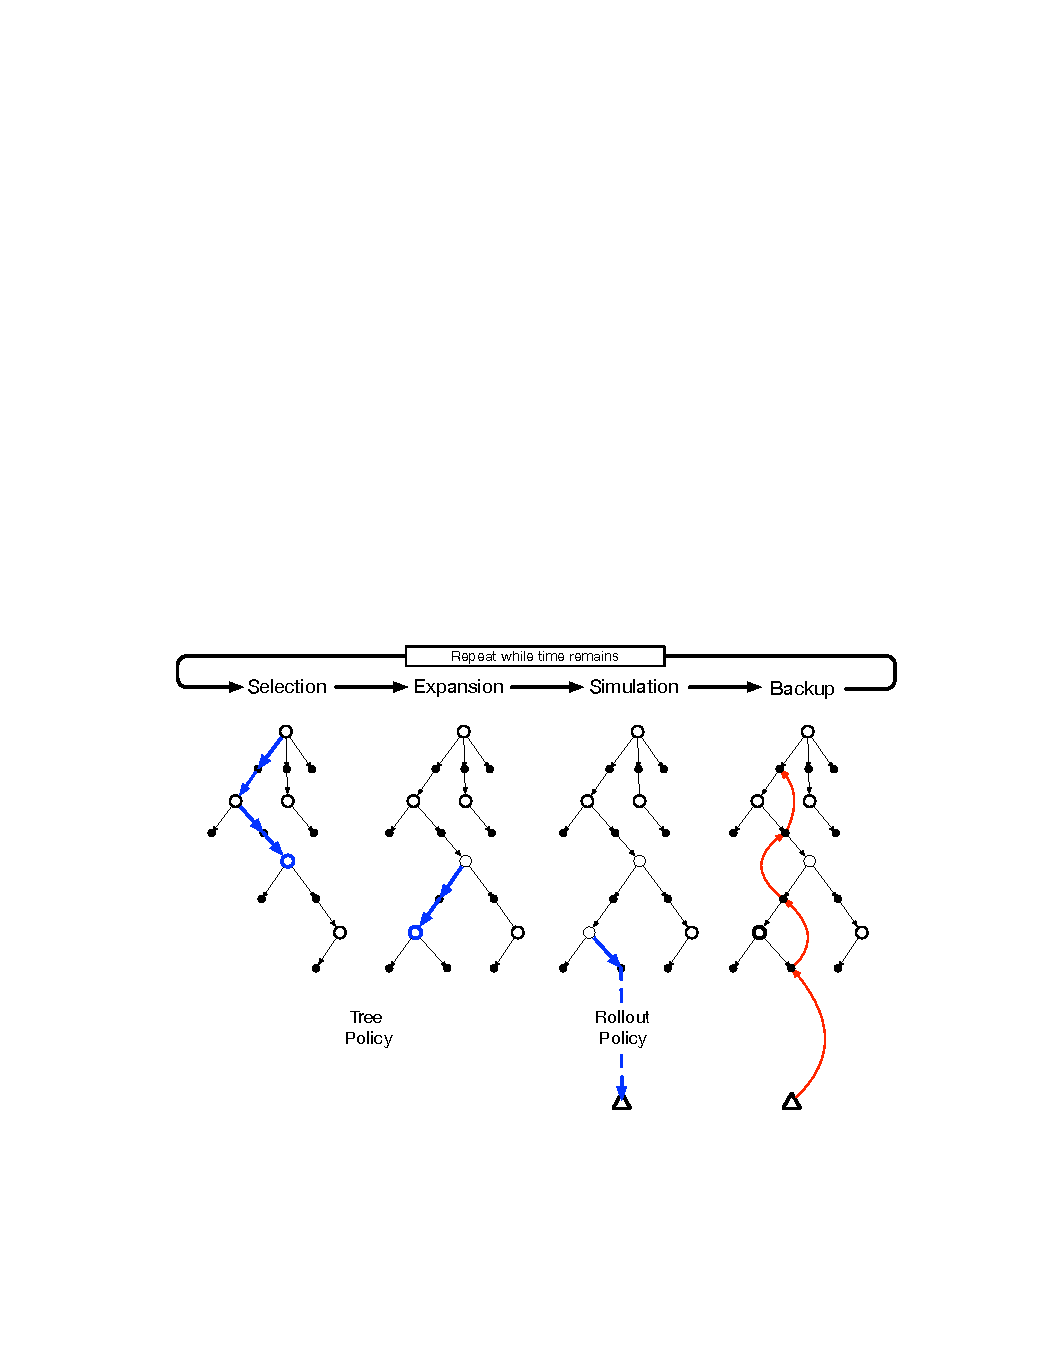
\includegraphics[width=8cm]{fig/lec07/MCTS.pdf}
	\caption{Basic building blocks of MCTS algorithms (source: R. Sutton and G. Barto, Reinforcement learning: an introduction, 2018, \href{https://creativecommons.org/licenses/by-nc-nd/2.0/}{CC BY-NC-ND 2.0})}
	\label{fig:MCTS}
\end{figure}
}

%%%%%%%%%%%%%%%%%%%%%%%%%%%%%%%%%%%%%%%%%%%%%%%%%%%%%%%%%%%%%
%% Basic MCTS Procedure %%
%%%%%%%%%%%%%%%%%%%%%%%%%%%%%%%%%%%%%%%%%%%%%%%%%%%%%%%%%%%%%
\frame{\frametitle{Basic MCTS Procedure}
Repeat the following steps while prediction time is available:
\begin{enumerate}
	\item \hl{Selection}: Starting at root node, use a tree policy (e.g., $\varepsilon$-greedy) to travel through the tree until arriving at a leaf node.\pause
	\begin{itemize}
		\item The tree policy exploits auspicious tree regions while maintaining some exploration.
		\item It is improved and (possibly) extended in every simulation run. \pause
	\end{itemize}
	\item \hl{Expansion}: Add child node(s) to the leaf node by evaluating unexplored actions (optional step). \pause
	\item \hl{Simulation}: Simulate the remaining full episode using the rollout policy starting from the leaf or child node (if available). \pause
	\begin{itemize}
		\item The rollout policy could be random, pre-trained or based on model-free methods using real experience (if available). \pause
	\end{itemize}
	\item \hl{Backup}: Update the values along the traveled trajectory but only saves those within the tree policy. 
\end{enumerate}
}

%%%%%%%%%%%%%%%%%%%%%%%%%%%%%%%%%%%%%%%%%%%%%%%%%%%%%%%%%%%%%
%% Further MCTS Remarks %%
%%%%%%%%%%%%%%%%%%%%%%%%%%%%%%%%%%%%%%%%%%%%%%%%%%%%%%%%%%%%%
\frame{\frametitle{Further MCTS Remarks}
What is happening after reaching the feasible simulation runs?
\begin{itemize}
	\item After time is up, MCTS picks an appropriate action regarding the root node, e.g.:
	\begin{itemize}
		\item The action visited the most times during all simulation runs or
		\item The action having the largest action value. \pause
	\end{itemize}
	\item After transitioning to a new state, the MCTS procedure re-starts:
	\begin{itemize}
		\item Either with a new tree incorporating only the root node or
		\item by re-utilizing the applicable parts from the previous tree. \pause
	\end{itemize}
\end{itemize}
\vspace{0.5cm}
Further reading on MCTS:
\begin{itemize}
	\item MCTS-based algorithms are not limited to game applications but were able to achieve outstanding success in this field.
	\begin{itemize}
		\item Famous AlphaGo (cf. \href{https://www.youtube.com/watch?v=Wujy7OzvdJk}{Keynote lecture from D. Silver})\pause
	\end{itemize}
	\item More in-depth lectures on MCTS can be found (among others) here:
	\begin{itemize}
		\item \href{https://www.youtube.com/watch?v=vDF1BYWhqL8}{Stanford Online: CS234}
		\item \href{https://www.youtube.com/watch?v=xmImNoDc9Z4}{MIT OpenCourseWare}
		\item \href{https://www.lri.fr/~sebag/Slides/InvitedTutorial_CP12.pdf}{Extensive slide set from M. Sebag at Universite Paris Sud}
	\end{itemize}
\end{itemize}
}

%%%%%%%%%%%%%%%%%%%%%%%%%%%%%%%%%%%%%%%%%%%%%%%%%%%%%%%%%%%%%
%% Summary %%
%%%%%%%%%%%%%%%%%%%%%%%%%%%%%%%%%%%%%%%%%%%%%%%%%%%%%%%%%%%%%
\begin{frame}
\frametitle{Summary: What You've Learned Today}
\begin{itemize}
	\item Model-free RL is easy to implement and cannot suffer any model learning error while model-based approaches use a limited amount of experience much more efficient. \pause
	\item Integrating these two RL branches can be achieved using the Dyna framework (background planning) incorporating the steps:
	\begin{itemize}
		\item Direct RL updates (any model-free approach, e.g., $Q$-learning),
		\item Model learning: use real experience to improve model predictions,
		\item Search control: strategies on how to generate simulated experience. \pause
	\end{itemize}
	\item The Dyna framework allows many different algorithms such as Dyna-$Q$(+) or prioritized sweeping.
	\begin{itemize}
		\item Learning efficiency is much increased compared to pure model-based/free approaches.
		\item Many degrees of freedom regarding internal update rules exist.\pause 
	\end{itemize}
	\item In contrast, planning at decision time predicts future trajectories starting from the current state (forward view).
	\begin{itemize}
		\item Rather computationally expensive leading to high latency responses.
		\item The Monte Carlo tree search rollout algorithm is a well-known example.
	\end{itemize}
\end{itemize}
\end{frame}

%%%%%%%%%%%%%%%%%%%%%%%%%%%%%%%%%%%%%%%%%%%%%%%%%%%%%%%%%%%%%
%% Final Slide %%
%%%%%%%%%%%%%%%%%%%%%%%%%%%%%%%%%%%%%%%%%%%%%%%%%%%%%%%%%%%%%
\frame{\frametitle{The End for Today}
\vspace{-0.25cm}
\begin{figure}
\hspace*{-0.5cm}
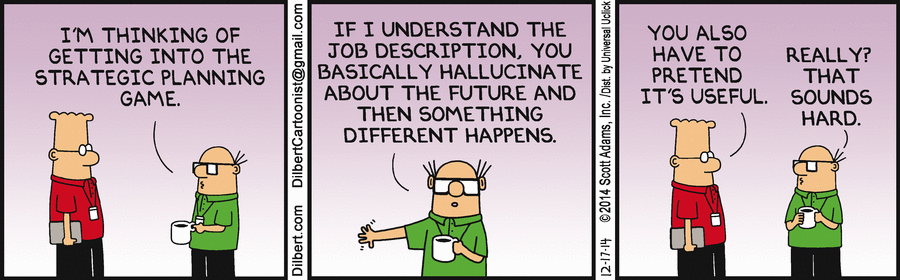
\includegraphics[width=10cm]{fig/lec07/dilbert.png}
\end{figure}
\vspace{1cm}
\centering
Thanks for your attention and have a nice week!
}